\documentclass[twoside]{book}

% Packages required by doxygen
\usepackage{fixltx2e}
\usepackage{calc}
\usepackage{doxygen}
\usepackage[export]{adjustbox} % also loads graphicx
\usepackage{graphicx}
\usepackage[utf8]{inputenc}
\usepackage{makeidx}
\usepackage{multicol}
\usepackage{multirow}
\PassOptionsToPackage{warn}{textcomp}
\usepackage{textcomp}
\usepackage[nointegrals]{wasysym}
\usepackage[table]{xcolor}

% Font selection
\usepackage[T1]{fontenc}
\usepackage[scaled=.90]{helvet}
\usepackage{courier}
\usepackage{amssymb}
\usepackage{sectsty}
\renewcommand{\familydefault}{\sfdefault}
\allsectionsfont{%
  \fontseries{bc}\selectfont%
  \color{darkgray}%
}
\renewcommand{\DoxyLabelFont}{%
  \fontseries{bc}\selectfont%
  \color{darkgray}%
}
\newcommand{\+}{\discretionary{\mbox{\scriptsize$\hookleftarrow$}}{}{}}

% Page & text layout
\usepackage{geometry}
\geometry{%
  a4paper,%
  top=2.5cm,%
  bottom=2.5cm,%
  left=2.5cm,%
  right=2.5cm%
}
\tolerance=750
\hfuzz=15pt
\hbadness=750
\setlength{\emergencystretch}{15pt}
\setlength{\parindent}{0cm}
\setlength{\parskip}{3ex plus 2ex minus 2ex}
\makeatletter
\renewcommand{\paragraph}{%
  \@startsection{paragraph}{4}{0ex}{-1.0ex}{1.0ex}{%
    \normalfont\normalsize\bfseries\SS@parafont%
  }%
}
\renewcommand{\subparagraph}{%
  \@startsection{subparagraph}{5}{0ex}{-1.0ex}{1.0ex}{%
    \normalfont\normalsize\bfseries\SS@subparafont%
  }%
}
\makeatother

% Headers & footers
\usepackage{fancyhdr}
\pagestyle{fancyplain}
\fancyhead[LE]{\fancyplain{}{\bfseries\thepage}}
\fancyhead[CE]{\fancyplain{}{}}
\fancyhead[RE]{\fancyplain{}{\bfseries\leftmark}}
\fancyhead[LO]{\fancyplain{}{\bfseries\rightmark}}
\fancyhead[CO]{\fancyplain{}{}}
\fancyhead[RO]{\fancyplain{}{\bfseries\thepage}}
\fancyfoot[LE]{\fancyplain{}{}}
\fancyfoot[CE]{\fancyplain{}{}}
\fancyfoot[RE]{\fancyplain{}{\bfseries\scriptsize Generated by Doxygen }}
\fancyfoot[LO]{\fancyplain{}{\bfseries\scriptsize Generated by Doxygen }}
\fancyfoot[CO]{\fancyplain{}{}}
\fancyfoot[RO]{\fancyplain{}{}}
\renewcommand{\footrulewidth}{0.4pt}
\renewcommand{\chaptermark}[1]{%
  \markboth{#1}{}%
}
\renewcommand{\sectionmark}[1]{%
  \markright{\thesection\ #1}%
}

% Indices & bibliography
\usepackage{natbib}
\usepackage[titles]{tocloft}
\setcounter{tocdepth}{3}
\setcounter{secnumdepth}{5}
\makeindex

% Hyperlinks (required, but should be loaded last)
\usepackage{ifpdf}
\ifpdf
  \usepackage[pdftex,pagebackref=true]{hyperref}
\else
  \usepackage[ps2pdf,pagebackref=true]{hyperref}
\fi
\hypersetup{%
  colorlinks=true,%
  linkcolor=blue,%
  citecolor=blue,%
  unicode%
}

% Custom commands
\newcommand{\clearemptydoublepage}{%
  \newpage{\pagestyle{empty}\cleardoublepage}%
}

\usepackage{caption}
\captionsetup{labelsep=space,justification=centering,font={bf},singlelinecheck=off,skip=4pt,position=top}

%===== C O N T E N T S =====

\begin{document}

% Titlepage & ToC
\hypersetup{pageanchor=false,
             bookmarksnumbered=true,
             pdfencoding=unicode
            }
\pagenumbering{alph}
\begin{titlepage}
\vspace*{7cm}
\begin{center}%
{\Large Pencil\+Producer }\\
\vspace*{1cm}
{\large Generated by Doxygen 1.8.13}\\
\end{center}
\end{titlepage}
\clearemptydoublepage
\pagenumbering{roman}
\tableofcontents
\clearemptydoublepage
\pagenumbering{arabic}
\hypersetup{pageanchor=true}

%--- Begin generated contents ---
\chapter{Pencil Producer}
\label{index}\hypertarget{index}{}\hypertarget{index_intro_sec}{}\section{Introduction}\label{index_intro_sec}
This project implements a pencil producer game where the player can produce and sell pencils to the public. In order to produce pencils the player must buy materials (wood, graphite). The player can increase and decrease the price of pencils at any point, which decreases and increases the demand for pencils respectively. \hypertarget{index_compile_sec}{}\section{Compilation}\label{index_compile_sec}

\begin{DoxyCode}
$ cd se-02-team/Pencil-Producer/

$ mkdir build

$ cd build/

$ cmake .. & make

$ ./pencilproducer
\end{DoxyCode}
 
\chapter{Namespace Index}
\section{Namespace List}
Here is a list of all namespaces with brief descriptions\+:\begin{DoxyCompactList}
\item\contentsline{section}{\hyperlink{namespaceUi}{Ui} }{\pageref{namespaceUi}}{}
\end{DoxyCompactList}

\chapter{Hierarchical Index}
\section{Class Hierarchy}
This inheritance list is sorted roughly, but not completely, alphabetically\+:\begin{DoxyCompactList}
\item \contentsline{section}{A\+P\+M2000\+\_\+\+Inventory}{\pageref{classAPM2000__Inventory}}{}
\item \contentsline{section}{Material\+\_\+\+Inventory}{\pageref{classMaterial__Inventory}}{}
\begin{DoxyCompactList}
\item \contentsline{section}{Graphite\+\_\+\+Inventory}{\pageref{classGraphite__Inventory}}{}
\item \contentsline{section}{Wood\+\_\+\+Inventory}{\pageref{classWood__Inventory}}{}
\end{DoxyCompactList}
\item \contentsline{section}{Pencil\+\_\+\+Inventory}{\pageref{classPencil__Inventory}}{}
\item Q\+Main\+Window\begin{DoxyCompactList}
\item \contentsline{section}{Pencil\+Producer}{\pageref{classPencilProducer}}{}
\end{DoxyCompactList}
\item Q\+Object\begin{DoxyCompactList}
\item \contentsline{section}{\+\_\+\+Test}{\pageref{class__Test}}{}
\end{DoxyCompactList}
\item \contentsline{section}{Wallet}{\pageref{classWallet}}{}
\end{DoxyCompactList}

\chapter{Class Index}
\section{Class List}
Here are the classes, structs, unions and interfaces with brief descriptions\+:\begin{DoxyCompactList}
\item\contentsline{section}{\hyperlink{class__Test}{\+\_\+\+Test} \\*The \hyperlink{class__Test}{\+\_\+\+Test} class main testing class }{\pageref{class__Test}}{}
\item\contentsline{section}{\hyperlink{classAPM2000__Inventory}{A\+P\+M2000\+\_\+\+Inventory} \\*The \hyperlink{classAPM2000__Inventory}{A\+P\+M2000\+\_\+\+Inventory} class Automatic Pencil Machine(\+A\+P\+M)~\newline
Suffix \char`\"{}2000\char`\"{} indicates 2000-\/series. Every 2000-\/series produces 2 pencils per second, which are automatically added into the inventory. A\+PM stops automatically when there are insufficient materials and resumes when materials are available }{\pageref{classAPM2000__Inventory}}{}
\item\contentsline{section}{\hyperlink{classGraphite__Inventory}{Graphite\+\_\+\+Inventory} }{\pageref{classGraphite__Inventory}}{}
\item\contentsline{section}{\hyperlink{classMaterial__Inventory}{Material\+\_\+\+Inventory} \\*The \hyperlink{classMaterial__Inventory}{Material\+\_\+\+Inventory} class superclass of other material classes }{\pageref{classMaterial__Inventory}}{}
\item\contentsline{section}{\hyperlink{classPencil__Inventory}{Pencil\+\_\+\+Inventory} \\*The \hyperlink{classPencil__Inventory}{Pencil\+\_\+\+Inventory} class main class for managing pencil prices and production }{\pageref{classPencil__Inventory}}{}
\item\contentsline{section}{\hyperlink{classPencilProducer}{Pencil\+Producer} \\*Class to implement the Pencil Producer game  In this class we will define the constructor/descructor and all the other methods we need to make it run. As for the first Spring, we are in need of a cons/dest only }{\pageref{classPencilProducer}}{}
\item\contentsline{section}{\hyperlink{classWallet}{Wallet} \\*The \hyperlink{classWallet}{Wallet} class keeps track of bank balance and methods for crediting/debiting account }{\pageref{classWallet}}{}
\item\contentsline{section}{\hyperlink{classWood__Inventory}{Wood\+\_\+\+Inventory} }{\pageref{classWood__Inventory}}{}
\end{DoxyCompactList}

\chapter{File Index}
\section{File List}
Here is a list of all files with brief descriptions\+:\begin{DoxyCompactList}
\item\contentsline{section}{/mnt/0896595996594878/\+Users/\+Maverick/\+Documents/\+University/\+School/\+Modules/4th Semester/\+Applied Computer Science/\+Software Eng/\+Project/\+Sprint\+\_\+02/se-\/02-\/team-\/09/\+Pencil-\/\+Producer/\hyperlink{apm2000__inventory_8cpp}{apm2000\+\_\+inventory.\+cpp} }{\pageref{apm2000__inventory_8cpp}}{}
\item\contentsline{section}{/mnt/0896595996594878/\+Users/\+Maverick/\+Documents/\+University/\+School/\+Modules/4th Semester/\+Applied Computer Science/\+Software Eng/\+Project/\+Sprint\+\_\+02/se-\/02-\/team-\/09/\+Pencil-\/\+Producer/\hyperlink{apm2000__inventory_8h}{apm2000\+\_\+inventory.\+h} }{\pageref{apm2000__inventory_8h}}{}
\item\contentsline{section}{/mnt/0896595996594878/\+Users/\+Maverick/\+Documents/\+University/\+School/\+Modules/4th Semester/\+Applied Computer Science/\+Software Eng/\+Project/\+Sprint\+\_\+02/se-\/02-\/team-\/09/\+Pencil-\/\+Producer/\hyperlink{graphite__inventory_8cpp}{graphite\+\_\+inventory.\+cpp} }{\pageref{graphite__inventory_8cpp}}{}
\item\contentsline{section}{/mnt/0896595996594878/\+Users/\+Maverick/\+Documents/\+University/\+School/\+Modules/4th Semester/\+Applied Computer Science/\+Software Eng/\+Project/\+Sprint\+\_\+02/se-\/02-\/team-\/09/\+Pencil-\/\+Producer/\hyperlink{graphite__inventory_8h}{graphite\+\_\+inventory.\+h} }{\pageref{graphite__inventory_8h}}{}
\item\contentsline{section}{/mnt/0896595996594878/\+Users/\+Maverick/\+Documents/\+University/\+School/\+Modules/4th Semester/\+Applied Computer Science/\+Software Eng/\+Project/\+Sprint\+\_\+02/se-\/02-\/team-\/09/\+Pencil-\/\+Producer/\hyperlink{main_8cpp}{main.\+cpp} }{\pageref{main_8cpp}}{}
\item\contentsline{section}{/mnt/0896595996594878/\+Users/\+Maverick/\+Documents/\+University/\+School/\+Modules/4th Semester/\+Applied Computer Science/\+Software Eng/\+Project/\+Sprint\+\_\+02/se-\/02-\/team-\/09/\+Pencil-\/\+Producer/\hyperlink{material__inventory_8cpp}{material\+\_\+inventory.\+cpp} }{\pageref{material__inventory_8cpp}}{}
\item\contentsline{section}{/mnt/0896595996594878/\+Users/\+Maverick/\+Documents/\+University/\+School/\+Modules/4th Semester/\+Applied Computer Science/\+Software Eng/\+Project/\+Sprint\+\_\+02/se-\/02-\/team-\/09/\+Pencil-\/\+Producer/\hyperlink{material__inventory_8h}{material\+\_\+inventory.\+h} }{\pageref{material__inventory_8h}}{}
\item\contentsline{section}{/mnt/0896595996594878/\+Users/\+Maverick/\+Documents/\+University/\+School/\+Modules/4th Semester/\+Applied Computer Science/\+Software Eng/\+Project/\+Sprint\+\_\+02/se-\/02-\/team-\/09/\+Pencil-\/\+Producer/\hyperlink{pencil__inventory_8cpp}{pencil\+\_\+inventory.\+cpp} }{\pageref{pencil__inventory_8cpp}}{}
\item\contentsline{section}{/mnt/0896595996594878/\+Users/\+Maverick/\+Documents/\+University/\+School/\+Modules/4th Semester/\+Applied Computer Science/\+Software Eng/\+Project/\+Sprint\+\_\+02/se-\/02-\/team-\/09/\+Pencil-\/\+Producer/\hyperlink{pencil__inventory_8h}{pencil\+\_\+inventory.\+h} }{\pageref{pencil__inventory_8h}}{}
\item\contentsline{section}{/mnt/0896595996594878/\+Users/\+Maverick/\+Documents/\+University/\+School/\+Modules/4th Semester/\+Applied Computer Science/\+Software Eng/\+Project/\+Sprint\+\_\+02/se-\/02-\/team-\/09/\+Pencil-\/\+Producer/\hyperlink{pencilproducer_8cpp}{pencilproducer.\+cpp} }{\pageref{pencilproducer_8cpp}}{}
\item\contentsline{section}{/mnt/0896595996594878/\+Users/\+Maverick/\+Documents/\+University/\+School/\+Modules/4th Semester/\+Applied Computer Science/\+Software Eng/\+Project/\+Sprint\+\_\+02/se-\/02-\/team-\/09/\+Pencil-\/\+Producer/\hyperlink{pencilproducer_8h}{pencilproducer.\+h} }{\pageref{pencilproducer_8h}}{}
\item\contentsline{section}{/mnt/0896595996594878/\+Users/\+Maverick/\+Documents/\+University/\+School/\+Modules/4th Semester/\+Applied Computer Science/\+Software Eng/\+Project/\+Sprint\+\_\+02/se-\/02-\/team-\/09/\+Pencil-\/\+Producer/\hyperlink{wallet_8cpp}{wallet.\+cpp} }{\pageref{wallet_8cpp}}{}
\item\contentsline{section}{/mnt/0896595996594878/\+Users/\+Maverick/\+Documents/\+University/\+School/\+Modules/4th Semester/\+Applied Computer Science/\+Software Eng/\+Project/\+Sprint\+\_\+02/se-\/02-\/team-\/09/\+Pencil-\/\+Producer/\hyperlink{wallet_8h}{wallet.\+h} }{\pageref{wallet_8h}}{}
\item\contentsline{section}{/mnt/0896595996594878/\+Users/\+Maverick/\+Documents/\+University/\+School/\+Modules/4th Semester/\+Applied Computer Science/\+Software Eng/\+Project/\+Sprint\+\_\+02/se-\/02-\/team-\/09/\+Pencil-\/\+Producer/\hyperlink{wood__inventory_8cpp}{wood\+\_\+inventory.\+cpp} }{\pageref{wood__inventory_8cpp}}{}
\item\contentsline{section}{/mnt/0896595996594878/\+Users/\+Maverick/\+Documents/\+University/\+School/\+Modules/4th Semester/\+Applied Computer Science/\+Software Eng/\+Project/\+Sprint\+\_\+02/se-\/02-\/team-\/09/\+Pencil-\/\+Producer/\hyperlink{wood__inventory_8h}{wood\+\_\+inventory.\+h} }{\pageref{wood__inventory_8h}}{}
\item\contentsline{section}{/mnt/0896595996594878/\+Users/\+Maverick/\+Documents/\+University/\+School/\+Modules/4th Semester/\+Applied Computer Science/\+Software Eng/\+Project/\+Sprint\+\_\+02/se-\/02-\/team-\/09/\+Test/\hyperlink{tst__test_8cpp}{tst\+\_\+test.\+cpp} }{\pageref{tst__test_8cpp}}{}
\end{DoxyCompactList}

\chapter{Namespace Documentation}
\hypertarget{namespaceUi}{}\section{Ui Namespace Reference}
\label{namespaceUi}\index{Ui@{Ui}}

\chapter{Class Documentation}
\hypertarget{class__Test}{}\section{\+\_\+\+Test Class Reference}
\label{class__Test}\index{\+\_\+\+Test@{\+\_\+\+Test}}


The \hyperlink{class__Test}{\+\_\+\+Test} class main testing class.  


Inheritance diagram for \+\_\+\+Test\+:\begin{figure}[H]
\begin{center}
\leavevmode
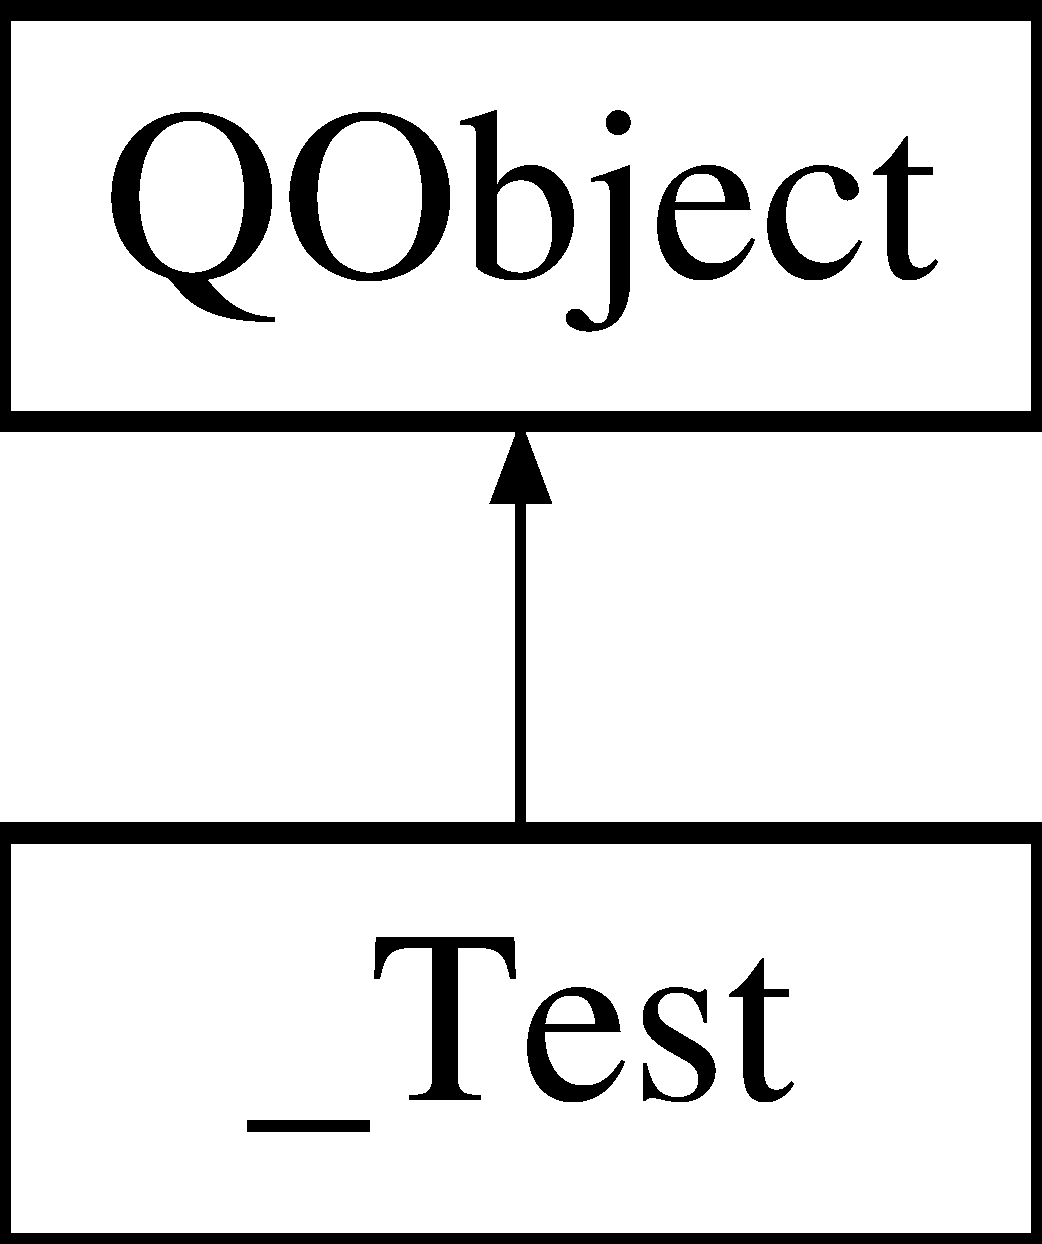
\includegraphics[height=2.000000cm]{class__Test}
\end{center}
\end{figure}
\subsection*{Public Member Functions}
\begin{DoxyCompactItemize}
\item 
\hyperlink{class__Test_a03ecfe4fd048c42338c5c54f73d830e2}{\+\_\+\+Test} ()
\item 
\hyperlink{class__Test_ac861d8bc0d139b86c2f30528d8c1bbbc}{$\sim$\+\_\+\+Test} ()
\end{DoxyCompactItemize}
\subsection*{Private Slots}
\begin{DoxyCompactItemize}
\item 
void \hyperlink{class__Test_a9cabdf9e5c265487d99174166d9206ff}{changing\+Pencil\+Price} ()
\item 
void \hyperlink{class__Test_a92dbc86899cfc80c08981ddcace05b5e}{sell\+Pencils} ()
\begin{DoxyCompactList}\small\item\em \+\_\+\+Test\+Pencil\+Invetory\+::sell\+Pencils test case for producing and selling pencils \end{DoxyCompactList}\item 
void \hyperlink{class__Test_afbce4b6817db0c8423dd4296a18f75de}{test\+Wallet} ()
\begin{DoxyCompactList}\small\item\em \hyperlink{class__Test_afbce4b6817db0c8423dd4296a18f75de}{\+\_\+\+Test\+::test\+Wallet} tests the functionality of the wallet class \end{DoxyCompactList}\item 
void \hyperlink{class__Test_adb7f71ea12e1b02afd6b4d1f7d65c1eb}{test\+A\+PM} ()
\begin{DoxyCompactList}\small\item\em \hyperlink{class__Test_adb7f71ea12e1b02afd6b4d1f7d65c1eb}{\+\_\+\+Test\+::test\+A\+PM} tests the functionality of the \hyperlink{classAPM2000__Inventory}{A\+P\+M2000\+\_\+\+Inventory} class \end{DoxyCompactList}\item 
void \hyperlink{class__Test_ad5396e54792008660924db2e16edb614}{test\+Materials} ()
\begin{DoxyCompactList}\small\item\em \hyperlink{class__Test_ad5396e54792008660924db2e16edb614}{\+\_\+\+Test\+::test\+Materials} tests the functionality of the material\+\_\+inventory superclass \end{DoxyCompactList}\end{DoxyCompactItemize}


\subsection{Detailed Description}
The \hyperlink{class__Test}{\+\_\+\+Test} class main testing class. 

\subsection{Constructor \& Destructor Documentation}
\mbox{\Hypertarget{class__Test_a03ecfe4fd048c42338c5c54f73d830e2}\label{class__Test_a03ecfe4fd048c42338c5c54f73d830e2}} 
\index{\+\_\+\+Test@{\+\_\+\+Test}!\+\_\+\+Test@{\+\_\+\+Test}}
\index{\+\_\+\+Test@{\+\_\+\+Test}!\+\_\+\+Test@{\+\_\+\+Test}}
\subsubsection{\texorpdfstring{\+\_\+\+Test()}{\_Test()}}
{\footnotesize\ttfamily \+\_\+\+Test\+::\+\_\+\+Test (\begin{DoxyParamCaption}{ }\end{DoxyParamCaption})}

\mbox{\Hypertarget{class__Test_ac861d8bc0d139b86c2f30528d8c1bbbc}\label{class__Test_ac861d8bc0d139b86c2f30528d8c1bbbc}} 
\index{\+\_\+\+Test@{\+\_\+\+Test}!````~\+\_\+\+Test@{$\sim$\+\_\+\+Test}}
\index{````~\+\_\+\+Test@{$\sim$\+\_\+\+Test}!\+\_\+\+Test@{\+\_\+\+Test}}
\subsubsection{\texorpdfstring{$\sim$\+\_\+\+Test()}{~\_Test()}}
{\footnotesize\ttfamily \+\_\+\+Test\+::$\sim$\+\_\+\+Test (\begin{DoxyParamCaption}{ }\end{DoxyParamCaption})}



\subsection{Member Function Documentation}
\mbox{\Hypertarget{class__Test_a9cabdf9e5c265487d99174166d9206ff}\label{class__Test_a9cabdf9e5c265487d99174166d9206ff}} 
\index{\+\_\+\+Test@{\+\_\+\+Test}!changing\+Pencil\+Price@{changing\+Pencil\+Price}}
\index{changing\+Pencil\+Price@{changing\+Pencil\+Price}!\+\_\+\+Test@{\+\_\+\+Test}}
\subsubsection{\texorpdfstring{changing\+Pencil\+Price}{changingPencilPrice}}
{\footnotesize\ttfamily void \+\_\+\+Test\+::changing\+Pencil\+Price (\begin{DoxyParamCaption}{ }\end{DoxyParamCaption})\hspace{0.3cm}{\ttfamily [private]}, {\ttfamily [slot]}}

\mbox{\Hypertarget{class__Test_a92dbc86899cfc80c08981ddcace05b5e}\label{class__Test_a92dbc86899cfc80c08981ddcace05b5e}} 
\index{\+\_\+\+Test@{\+\_\+\+Test}!sell\+Pencils@{sell\+Pencils}}
\index{sell\+Pencils@{sell\+Pencils}!\+\_\+\+Test@{\+\_\+\+Test}}
\subsubsection{\texorpdfstring{sell\+Pencils}{sellPencils}}
{\footnotesize\ttfamily void \+\_\+\+Test\+::sell\+Pencils (\begin{DoxyParamCaption}{ }\end{DoxyParamCaption})\hspace{0.3cm}{\ttfamily [private]}, {\ttfamily [slot]}}



\+\_\+\+Test\+Pencil\+Invetory\+::sell\+Pencils test case for producing and selling pencils 

\mbox{\Hypertarget{class__Test_adb7f71ea12e1b02afd6b4d1f7d65c1eb}\label{class__Test_adb7f71ea12e1b02afd6b4d1f7d65c1eb}} 
\index{\+\_\+\+Test@{\+\_\+\+Test}!test\+A\+PM@{test\+A\+PM}}
\index{test\+A\+PM@{test\+A\+PM}!\+\_\+\+Test@{\+\_\+\+Test}}
\subsubsection{\texorpdfstring{test\+A\+PM}{testAPM}}
{\footnotesize\ttfamily void \+\_\+\+Test\+::test\+A\+PM (\begin{DoxyParamCaption}{ }\end{DoxyParamCaption})\hspace{0.3cm}{\ttfamily [private]}, {\ttfamily [slot]}}



\hyperlink{class__Test_adb7f71ea12e1b02afd6b4d1f7d65c1eb}{\+\_\+\+Test\+::test\+A\+PM} tests the functionality of the \hyperlink{classAPM2000__Inventory}{A\+P\+M2000\+\_\+\+Inventory} class 

\mbox{\Hypertarget{class__Test_ad5396e54792008660924db2e16edb614}\label{class__Test_ad5396e54792008660924db2e16edb614}} 
\index{\+\_\+\+Test@{\+\_\+\+Test}!test\+Materials@{test\+Materials}}
\index{test\+Materials@{test\+Materials}!\+\_\+\+Test@{\+\_\+\+Test}}
\subsubsection{\texorpdfstring{test\+Materials}{testMaterials}}
{\footnotesize\ttfamily void \+\_\+\+Test\+::test\+Materials (\begin{DoxyParamCaption}{ }\end{DoxyParamCaption})\hspace{0.3cm}{\ttfamily [private]}, {\ttfamily [slot]}}



\hyperlink{class__Test_ad5396e54792008660924db2e16edb614}{\+\_\+\+Test\+::test\+Materials} tests the functionality of the material\+\_\+inventory superclass 

\mbox{\Hypertarget{class__Test_afbce4b6817db0c8423dd4296a18f75de}\label{class__Test_afbce4b6817db0c8423dd4296a18f75de}} 
\index{\+\_\+\+Test@{\+\_\+\+Test}!test\+Wallet@{test\+Wallet}}
\index{test\+Wallet@{test\+Wallet}!\+\_\+\+Test@{\+\_\+\+Test}}
\subsubsection{\texorpdfstring{test\+Wallet}{testWallet}}
{\footnotesize\ttfamily void \+\_\+\+Test\+::test\+Wallet (\begin{DoxyParamCaption}{ }\end{DoxyParamCaption})\hspace{0.3cm}{\ttfamily [private]}, {\ttfamily [slot]}}



\hyperlink{class__Test_afbce4b6817db0c8423dd4296a18f75de}{\+\_\+\+Test\+::test\+Wallet} tests the functionality of the wallet class 



The documentation for this class was generated from the following file\+:\begin{DoxyCompactItemize}
\item 
/mnt/0896595996594878/\+Users/\+Maverick/\+Documents/\+University/\+School/\+Modules/4th Semester/\+Applied Computer Science/\+Software Eng/\+Project/\+Sprint\+\_\+02/se-\/02-\/team-\/09/\+Test/\hyperlink{tst__test_8cpp}{tst\+\_\+test.\+cpp}\end{DoxyCompactItemize}

\hypertarget{classAPM2000__Inventory}{}\section{A\+P\+M2000\+\_\+\+Inventory Class Reference}
\label{classAPM2000__Inventory}\index{A\+P\+M2000\+\_\+\+Inventory@{A\+P\+M2000\+\_\+\+Inventory}}


The \hyperlink{classAPM2000__Inventory}{A\+P\+M2000\+\_\+\+Inventory} class Automatic Pencil Machine(\+A\+P\+M)~\newline
Suffix \char`\"{}2000\char`\"{} indicates 2000-\/series. Every 2000-\/series produces 2 pencils per second, which are automatically added into the inventory. A\+PM stops automatically when there are insufficient materials and resumes when materials are available.  




{\ttfamily \#include $<$apm2000\+\_\+inventory.\+h$>$}

\subsection*{Public Member Functions}
\begin{DoxyCompactItemize}
\item 
\hyperlink{classAPM2000__Inventory_a0aa6a0abe496ccd0ee773c4a3ce38a2c}{A\+P\+M2000\+\_\+\+Inventory} ()
\begin{DoxyCompactList}\small\item\em \hyperlink{classAPM2000__Inventory_a0aa6a0abe496ccd0ee773c4a3ce38a2c}{A\+P\+M2000\+\_\+\+Inventory\+::\+A\+P\+M2000\+\_\+\+Inventory} \hyperlink{classAPM2000__Inventory}{A\+P\+M2000\+\_\+\+Inventory} constructor.~\newline
Default values\+:~\newline
number = 0~\newline
price = \$150.\+00. \end{DoxyCompactList}\item 
void \hyperlink{classAPM2000__Inventory_a5f89890fced248efa0792e0ac062e9e2}{buy\+A\+P\+M2000} (\hyperlink{classWallet}{Wallet} \&)
\begin{DoxyCompactList}\small\item\em \hyperlink{classAPM2000__Inventory_a5f89890fced248efa0792e0ac062e9e2}{A\+P\+M2000\+\_\+\+Inventory\+::buy\+A\+P\+M2000} If can\+Buy\+A\+P\+M2000 evaluates to true, bank balance is debited, the number of A\+P\+Ms in inventory increases by 1 and the A\+PM price is updated. \end{DoxyCompactList}\item 
bool \hyperlink{classAPM2000__Inventory_a8edb69c3a8614e7b709605f59a3c409b}{can\+Buy\+A\+P\+M2000} (\hyperlink{classWallet}{Wallet} \&)
\begin{DoxyCompactList}\small\item\em \hyperlink{classAPM2000__Inventory_a8edb69c3a8614e7b709605f59a3c409b}{A\+P\+M2000\+\_\+\+Inventory\+::can\+Buy\+A\+P\+M2000} checks if wallet balance has enough for new A\+PM and if the number of A\+P\+Ms in inventory is less than the max (10). \end{DoxyCompactList}\item 
void \hyperlink{classAPM2000__Inventory_ad7ffc7e7536509d26d76800b2398bfc0}{produce\+Pencil} (\hyperlink{classPencil__Inventory}{Pencil\+\_\+\+Inventory} \&, \hyperlink{classGraphite__Inventory}{Graphite\+\_\+\+Inventory} \&, \hyperlink{classWood__Inventory}{Wood\+\_\+\+Inventory} \&)
\item 
bool \hyperlink{classAPM2000__Inventory_a57eae269c4c67d3133175d6006373d2b}{can\+Produce\+Pencil} (\hyperlink{classPencil__Inventory}{Pencil\+\_\+\+Inventory} \&, \hyperlink{classGraphite__Inventory}{Graphite\+\_\+\+Inventory} \&, \hyperlink{classWood__Inventory}{Wood\+\_\+\+Inventory} \&)
\item 
int \hyperlink{classAPM2000__Inventory_a9a9bacffea28885b6c268d9a3bcab401}{get\+Number} () const
\begin{DoxyCompactList}\small\item\em returns number of A\+P\+Ms in inventory \end{DoxyCompactList}\item 
float \hyperlink{classAPM2000__Inventory_a65388780b7aa2066cfaf86c85d501765}{get\+Price} () const
\begin{DoxyCompactList}\small\item\em returns price of A\+PM \end{DoxyCompactList}\item 
int \hyperlink{classAPM2000__Inventory_ab20a0adafade1bdefea0e8d8c6b271a0}{get\+Rate} () const
\end{DoxyCompactItemize}
\subsection*{Private Attributes}
\begin{DoxyCompactItemize}
\item 
const int \hyperlink{classAPM2000__Inventory_a098109b5a53ce171fb405e552bf056b2}{max} = 10
\begin{DoxyCompactList}\small\item\em maximum number of A\+P\+Ms allowed \end{DoxyCompactList}\item 
int \hyperlink{classAPM2000__Inventory_a0393939ee2dd57ec3855bb98070da2ad}{number}
\begin{DoxyCompactList}\small\item\em number of A\+P\+Ms in your inventory \end{DoxyCompactList}\item 
float \hyperlink{classAPM2000__Inventory_a56588e2f627cbe3fccf6235773d77889}{price}
\begin{DoxyCompactList}\small\item\em price of A\+PM \end{DoxyCompactList}\end{DoxyCompactItemize}


\subsection{Detailed Description}
The \hyperlink{classAPM2000__Inventory}{A\+P\+M2000\+\_\+\+Inventory} class Automatic Pencil Machine(\+A\+P\+M)~\newline
Suffix \char`\"{}2000\char`\"{} indicates 2000-\/series. Every 2000-\/series produces 2 pencils per second, which are automatically added into the inventory. A\+PM stops automatically when there are insufficient materials and resumes when materials are available. 

\subsection{Constructor \& Destructor Documentation}
\mbox{\Hypertarget{classAPM2000__Inventory_a0aa6a0abe496ccd0ee773c4a3ce38a2c}\label{classAPM2000__Inventory_a0aa6a0abe496ccd0ee773c4a3ce38a2c}} 
\index{A\+P\+M2000\+\_\+\+Inventory@{A\+P\+M2000\+\_\+\+Inventory}!A\+P\+M2000\+\_\+\+Inventory@{A\+P\+M2000\+\_\+\+Inventory}}
\index{A\+P\+M2000\+\_\+\+Inventory@{A\+P\+M2000\+\_\+\+Inventory}!A\+P\+M2000\+\_\+\+Inventory@{A\+P\+M2000\+\_\+\+Inventory}}
\subsubsection{\texorpdfstring{A\+P\+M2000\+\_\+\+Inventory()}{APM2000\_Inventory()}}
{\footnotesize\ttfamily A\+P\+M2000\+\_\+\+Inventory\+::\+A\+P\+M2000\+\_\+\+Inventory (\begin{DoxyParamCaption}{ }\end{DoxyParamCaption})}



\hyperlink{classAPM2000__Inventory_a0aa6a0abe496ccd0ee773c4a3ce38a2c}{A\+P\+M2000\+\_\+\+Inventory\+::\+A\+P\+M2000\+\_\+\+Inventory} \hyperlink{classAPM2000__Inventory}{A\+P\+M2000\+\_\+\+Inventory} constructor.~\newline
Default values\+:~\newline
number = 0~\newline
price = \$150.\+00. 



\subsection{Member Function Documentation}
\mbox{\Hypertarget{classAPM2000__Inventory_a5f89890fced248efa0792e0ac062e9e2}\label{classAPM2000__Inventory_a5f89890fced248efa0792e0ac062e9e2}} 
\index{A\+P\+M2000\+\_\+\+Inventory@{A\+P\+M2000\+\_\+\+Inventory}!buy\+A\+P\+M2000@{buy\+A\+P\+M2000}}
\index{buy\+A\+P\+M2000@{buy\+A\+P\+M2000}!A\+P\+M2000\+\_\+\+Inventory@{A\+P\+M2000\+\_\+\+Inventory}}
\subsubsection{\texorpdfstring{buy\+A\+P\+M2000()}{buyAPM2000()}}
{\footnotesize\ttfamily void A\+P\+M2000\+\_\+\+Inventory\+::buy\+A\+P\+M2000 (\begin{DoxyParamCaption}\item[{\hyperlink{classWallet}{Wallet} \&}]{wallet }\end{DoxyParamCaption})}



\hyperlink{classAPM2000__Inventory_a5f89890fced248efa0792e0ac062e9e2}{A\+P\+M2000\+\_\+\+Inventory\+::buy\+A\+P\+M2000} If can\+Buy\+A\+P\+M2000 evaluates to true, bank balance is debited, the number of A\+P\+Ms in inventory increases by 1 and the A\+PM price is updated. 


\begin{DoxyParams}{Parameters}
{\em wallet} & \\
\hline
\end{DoxyParams}
\mbox{\Hypertarget{classAPM2000__Inventory_a8edb69c3a8614e7b709605f59a3c409b}\label{classAPM2000__Inventory_a8edb69c3a8614e7b709605f59a3c409b}} 
\index{A\+P\+M2000\+\_\+\+Inventory@{A\+P\+M2000\+\_\+\+Inventory}!can\+Buy\+A\+P\+M2000@{can\+Buy\+A\+P\+M2000}}
\index{can\+Buy\+A\+P\+M2000@{can\+Buy\+A\+P\+M2000}!A\+P\+M2000\+\_\+\+Inventory@{A\+P\+M2000\+\_\+\+Inventory}}
\subsubsection{\texorpdfstring{can\+Buy\+A\+P\+M2000()}{canBuyAPM2000()}}
{\footnotesize\ttfamily bool A\+P\+M2000\+\_\+\+Inventory\+::can\+Buy\+A\+P\+M2000 (\begin{DoxyParamCaption}\item[{\hyperlink{classWallet}{Wallet} \&}]{wallet }\end{DoxyParamCaption})}



\hyperlink{classAPM2000__Inventory_a8edb69c3a8614e7b709605f59a3c409b}{A\+P\+M2000\+\_\+\+Inventory\+::can\+Buy\+A\+P\+M2000} checks if wallet balance has enough for new A\+PM and if the number of A\+P\+Ms in inventory is less than the max (10). 


\begin{DoxyParams}{Parameters}
{\em wallet} & \\
\hline
\end{DoxyParams}
\begin{DoxyReturn}{Returns}
true conditions are met, false otherwise 
\end{DoxyReturn}
\mbox{\Hypertarget{classAPM2000__Inventory_a57eae269c4c67d3133175d6006373d2b}\label{classAPM2000__Inventory_a57eae269c4c67d3133175d6006373d2b}} 
\index{A\+P\+M2000\+\_\+\+Inventory@{A\+P\+M2000\+\_\+\+Inventory}!can\+Produce\+Pencil@{can\+Produce\+Pencil}}
\index{can\+Produce\+Pencil@{can\+Produce\+Pencil}!A\+P\+M2000\+\_\+\+Inventory@{A\+P\+M2000\+\_\+\+Inventory}}
\subsubsection{\texorpdfstring{can\+Produce\+Pencil()}{canProducePencil()}}
{\footnotesize\ttfamily bool A\+P\+M2000\+\_\+\+Inventory\+::can\+Produce\+Pencil (\begin{DoxyParamCaption}\item[{\hyperlink{classPencil__Inventory}{Pencil\+\_\+\+Inventory} \&}]{pencil\+Inventory,  }\item[{\hyperlink{classGraphite__Inventory}{Graphite\+\_\+\+Inventory} \&}]{graphite\+Inventory,  }\item[{\hyperlink{classWood__Inventory}{Wood\+\_\+\+Inventory} \&}]{wood\+Inventory }\end{DoxyParamCaption})}

\mbox{\Hypertarget{classAPM2000__Inventory_a9a9bacffea28885b6c268d9a3bcab401}\label{classAPM2000__Inventory_a9a9bacffea28885b6c268d9a3bcab401}} 
\index{A\+P\+M2000\+\_\+\+Inventory@{A\+P\+M2000\+\_\+\+Inventory}!get\+Number@{get\+Number}}
\index{get\+Number@{get\+Number}!A\+P\+M2000\+\_\+\+Inventory@{A\+P\+M2000\+\_\+\+Inventory}}
\subsubsection{\texorpdfstring{get\+Number()}{getNumber()}}
{\footnotesize\ttfamily int A\+P\+M2000\+\_\+\+Inventory\+::get\+Number (\begin{DoxyParamCaption}{ }\end{DoxyParamCaption}) const}



returns number of A\+P\+Ms in inventory 

\mbox{\Hypertarget{classAPM2000__Inventory_a65388780b7aa2066cfaf86c85d501765}\label{classAPM2000__Inventory_a65388780b7aa2066cfaf86c85d501765}} 
\index{A\+P\+M2000\+\_\+\+Inventory@{A\+P\+M2000\+\_\+\+Inventory}!get\+Price@{get\+Price}}
\index{get\+Price@{get\+Price}!A\+P\+M2000\+\_\+\+Inventory@{A\+P\+M2000\+\_\+\+Inventory}}
\subsubsection{\texorpdfstring{get\+Price()}{getPrice()}}
{\footnotesize\ttfamily float A\+P\+M2000\+\_\+\+Inventory\+::get\+Price (\begin{DoxyParamCaption}{ }\end{DoxyParamCaption}) const}



returns price of A\+PM 

\mbox{\Hypertarget{classAPM2000__Inventory_ab20a0adafade1bdefea0e8d8c6b271a0}\label{classAPM2000__Inventory_ab20a0adafade1bdefea0e8d8c6b271a0}} 
\index{A\+P\+M2000\+\_\+\+Inventory@{A\+P\+M2000\+\_\+\+Inventory}!get\+Rate@{get\+Rate}}
\index{get\+Rate@{get\+Rate}!A\+P\+M2000\+\_\+\+Inventory@{A\+P\+M2000\+\_\+\+Inventory}}
\subsubsection{\texorpdfstring{get\+Rate()}{getRate()}}
{\footnotesize\ttfamily int A\+P\+M2000\+\_\+\+Inventory\+::get\+Rate (\begin{DoxyParamCaption}{ }\end{DoxyParamCaption}) const}

\mbox{\Hypertarget{classAPM2000__Inventory_ad7ffc7e7536509d26d76800b2398bfc0}\label{classAPM2000__Inventory_ad7ffc7e7536509d26d76800b2398bfc0}} 
\index{A\+P\+M2000\+\_\+\+Inventory@{A\+P\+M2000\+\_\+\+Inventory}!produce\+Pencil@{produce\+Pencil}}
\index{produce\+Pencil@{produce\+Pencil}!A\+P\+M2000\+\_\+\+Inventory@{A\+P\+M2000\+\_\+\+Inventory}}
\subsubsection{\texorpdfstring{produce\+Pencil()}{producePencil()}}
{\footnotesize\ttfamily void A\+P\+M2000\+\_\+\+Inventory\+::produce\+Pencil (\begin{DoxyParamCaption}\item[{\hyperlink{classPencil__Inventory}{Pencil\+\_\+\+Inventory} \&}]{pencil\+Inventory,  }\item[{\hyperlink{classGraphite__Inventory}{Graphite\+\_\+\+Inventory} \&}]{graphite\+Inventory,  }\item[{\hyperlink{classWood__Inventory}{Wood\+\_\+\+Inventory} \&}]{wood\+Inventory }\end{DoxyParamCaption})}



\subsection{Member Data Documentation}
\mbox{\Hypertarget{classAPM2000__Inventory_a098109b5a53ce171fb405e552bf056b2}\label{classAPM2000__Inventory_a098109b5a53ce171fb405e552bf056b2}} 
\index{A\+P\+M2000\+\_\+\+Inventory@{A\+P\+M2000\+\_\+\+Inventory}!max@{max}}
\index{max@{max}!A\+P\+M2000\+\_\+\+Inventory@{A\+P\+M2000\+\_\+\+Inventory}}
\subsubsection{\texorpdfstring{max}{max}}
{\footnotesize\ttfamily const int A\+P\+M2000\+\_\+\+Inventory\+::max = 10\hspace{0.3cm}{\ttfamily [private]}}



maximum number of A\+P\+Ms allowed 

\mbox{\Hypertarget{classAPM2000__Inventory_a0393939ee2dd57ec3855bb98070da2ad}\label{classAPM2000__Inventory_a0393939ee2dd57ec3855bb98070da2ad}} 
\index{A\+P\+M2000\+\_\+\+Inventory@{A\+P\+M2000\+\_\+\+Inventory}!number@{number}}
\index{number@{number}!A\+P\+M2000\+\_\+\+Inventory@{A\+P\+M2000\+\_\+\+Inventory}}
\subsubsection{\texorpdfstring{number}{number}}
{\footnotesize\ttfamily int A\+P\+M2000\+\_\+\+Inventory\+::number\hspace{0.3cm}{\ttfamily [private]}}



number of A\+P\+Ms in your inventory 

\mbox{\Hypertarget{classAPM2000__Inventory_a56588e2f627cbe3fccf6235773d77889}\label{classAPM2000__Inventory_a56588e2f627cbe3fccf6235773d77889}} 
\index{A\+P\+M2000\+\_\+\+Inventory@{A\+P\+M2000\+\_\+\+Inventory}!price@{price}}
\index{price@{price}!A\+P\+M2000\+\_\+\+Inventory@{A\+P\+M2000\+\_\+\+Inventory}}
\subsubsection{\texorpdfstring{price}{price}}
{\footnotesize\ttfamily float A\+P\+M2000\+\_\+\+Inventory\+::price\hspace{0.3cm}{\ttfamily [private]}}



price of A\+PM 



The documentation for this class was generated from the following files\+:\begin{DoxyCompactItemize}
\item 
/mnt/0896595996594878/\+Users/\+Maverick/\+Documents/\+University/\+School/\+Modules/4th Semester/\+Applied Computer Science/\+Software Eng/\+Project/\+Sprint\+\_\+02/se-\/02-\/team-\/09/\+Pencil-\/\+Producer/\hyperlink{apm2000__inventory_8h}{apm2000\+\_\+inventory.\+h}\item 
/mnt/0896595996594878/\+Users/\+Maverick/\+Documents/\+University/\+School/\+Modules/4th Semester/\+Applied Computer Science/\+Software Eng/\+Project/\+Sprint\+\_\+02/se-\/02-\/team-\/09/\+Pencil-\/\+Producer/\hyperlink{apm2000__inventory_8cpp}{apm2000\+\_\+inventory.\+cpp}\end{DoxyCompactItemize}

\hypertarget{classGraphite__Inventory}{}\section{Graphite\+\_\+\+Inventory Class Reference}
\label{classGraphite__Inventory}\index{Graphite\+\_\+\+Inventory@{Graphite\+\_\+\+Inventory}}


{\ttfamily \#include $<$graphite\+\_\+inventory.\+h$>$}

Inheritance diagram for Graphite\+\_\+\+Inventory\+:\begin{figure}[H]
\begin{center}
\leavevmode
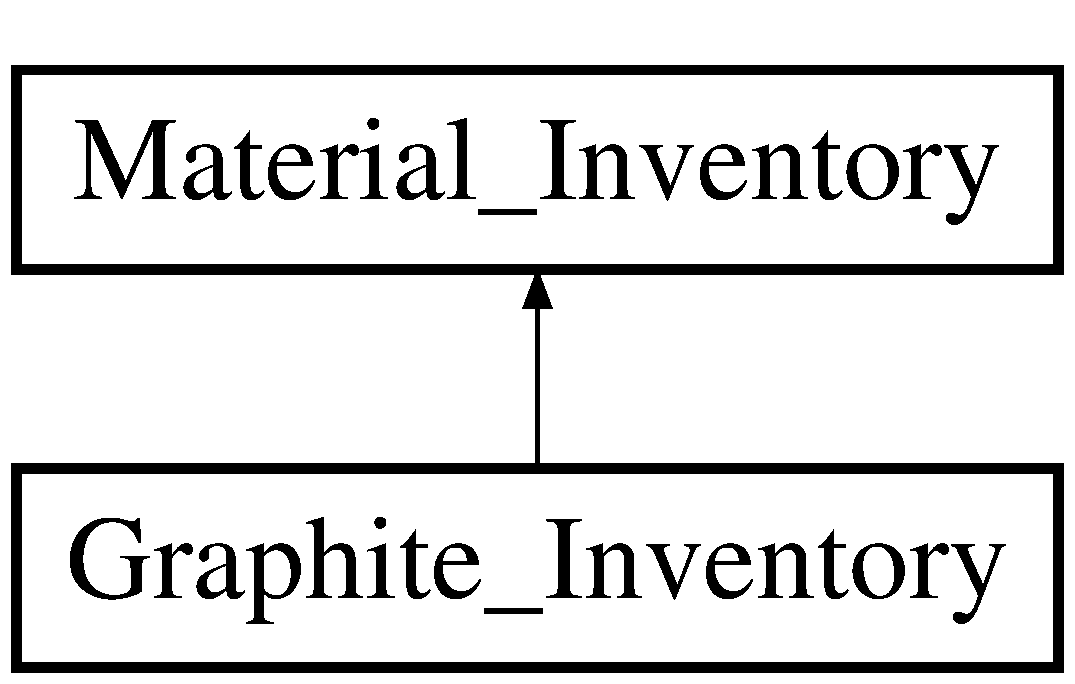
\includegraphics[height=2.000000cm]{classGraphite__Inventory}
\end{center}
\end{figure}
\subsection*{Public Member Functions}
\begin{DoxyCompactItemize}
\item 
\hyperlink{classGraphite__Inventory_aee64464327d4c5d6eb37d293fa83b5a6}{Graphite\+\_\+\+Inventory} ()
\end{DoxyCompactItemize}


\subsection{Constructor \& Destructor Documentation}
\mbox{\Hypertarget{classGraphite__Inventory_aee64464327d4c5d6eb37d293fa83b5a6}\label{classGraphite__Inventory_aee64464327d4c5d6eb37d293fa83b5a6}} 
\index{Graphite\+\_\+\+Inventory@{Graphite\+\_\+\+Inventory}!Graphite\+\_\+\+Inventory@{Graphite\+\_\+\+Inventory}}
\index{Graphite\+\_\+\+Inventory@{Graphite\+\_\+\+Inventory}!Graphite\+\_\+\+Inventory@{Graphite\+\_\+\+Inventory}}
\subsubsection{\texorpdfstring{Graphite\+\_\+\+Inventory()}{Graphite\_Inventory()}}
{\footnotesize\ttfamily Graphite\+\_\+\+Inventory\+::\+Graphite\+\_\+\+Inventory (\begin{DoxyParamCaption}{ }\end{DoxyParamCaption})}



The documentation for this class was generated from the following files\+:\begin{DoxyCompactItemize}
\item 
/mnt/0896595996594878/\+Users/\+Maverick/\+Documents/\+University/\+School/\+Modules/4th Semester/\+Applied Computer Science/\+Software Eng/\+Project/\+Sprint\+\_\+02/se-\/02-\/team-\/09/\+Pencil-\/\+Producer/\hyperlink{graphite__inventory_8h}{graphite\+\_\+inventory.\+h}\item 
/mnt/0896595996594878/\+Users/\+Maverick/\+Documents/\+University/\+School/\+Modules/4th Semester/\+Applied Computer Science/\+Software Eng/\+Project/\+Sprint\+\_\+02/se-\/02-\/team-\/09/\+Pencil-\/\+Producer/\hyperlink{graphite__inventory_8cpp}{graphite\+\_\+inventory.\+cpp}\end{DoxyCompactItemize}

\hypertarget{classMaterial__Inventory}{}\section{Material\+\_\+\+Inventory Class Reference}
\label{classMaterial__Inventory}\index{Material\+\_\+\+Inventory@{Material\+\_\+\+Inventory}}


The \hyperlink{classMaterial__Inventory}{Material\+\_\+\+Inventory} class superclass of other material classes.  




{\ttfamily \#include $<$material\+\_\+inventory.\+h$>$}

Inheritance diagram for Material\+\_\+\+Inventory\+:\begin{figure}[H]
\begin{center}
\leavevmode
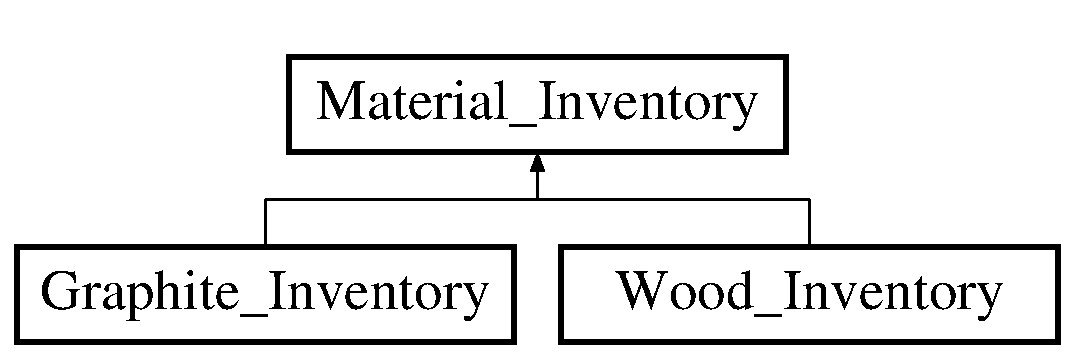
\includegraphics[height=2.000000cm]{classMaterial__Inventory}
\end{center}
\end{figure}
\subsection*{Public Member Functions}
\begin{DoxyCompactItemize}
\item 
\hyperlink{classMaterial__Inventory_a996e5441abe78653a8cb386a499a4063}{Material\+\_\+\+Inventory} (float, float)
\item 
void \hyperlink{classMaterial__Inventory_a5be24d53377c58ea2391e0f872d199d8}{buy} (\hyperlink{classWallet}{Wallet} \&)
\begin{DoxyCompactList}\small\item\em \hyperlink{classMaterial__Inventory_a5be24d53377c58ea2391e0f872d199d8}{Material\+\_\+\+Inventory\+::buy} if there are sufficient funds in bank balance, increase the amount of material in inventory by 100.\+00m and debit bank balance. \end{DoxyCompactList}\item 
bool \hyperlink{classMaterial__Inventory_abb1d889d0af7b79da3b5100a409a5140}{can\+Buy} (\hyperlink{classWallet}{Wallet} \&) const
\item 
float \hyperlink{classMaterial__Inventory_a3e3bf78a963137fdf3be88cecbdcb778}{get\+Price} () const
\begin{DoxyCompactList}\small\item\em returns price of material \end{DoxyCompactList}\item 
void \hyperlink{classMaterial__Inventory_a1ae3a7d9e3d42c8d5bfee551605722ee}{set\+Price} ()
\begin{DoxyCompactList}\small\item\em randomly increases the price of the material within a certain value range \end{DoxyCompactList}\item 
float \hyperlink{classMaterial__Inventory_acc6a2d2b8dc613689561b0165d591fb1}{get\+Amount} () const
\begin{DoxyCompactList}\small\item\em returns the amount of the material in inventory \end{DoxyCompactList}\item 
void \hyperlink{classMaterial__Inventory_a8c281edc32968e93c0a820ed29ccf3d5}{consume} (int n=1)
\begin{DoxyCompactList}\small\item\em \hyperlink{classMaterial__Inventory_a8c281edc32968e93c0a820ed29ccf3d5}{Material\+\_\+\+Inventory\+::consume} if there is sufficient material, reduces the amount of material in inventory by the appropriate amount. \end{DoxyCompactList}\item 
bool \hyperlink{classMaterial__Inventory_a21e999476b95f52063d222ef892887ba}{can\+Consume} (int n=1) const
\end{DoxyCompactItemize}
\subsection*{Private Attributes}
\begin{DoxyCompactItemize}
\item 
float \hyperlink{classMaterial__Inventory_a32622250fa5246e1ee091d3fd8dd72ff}{price}
\begin{DoxyCompactList}\small\item\em price of 100.\+00m of material \end{DoxyCompactList}\item 
float \hyperlink{classMaterial__Inventory_a928c45234f051861431e8adc1bd4f368}{amount}
\begin{DoxyCompactList}\small\item\em amount of material in inventory \end{DoxyCompactList}\item 
float \hyperlink{classMaterial__Inventory_afb28e18e6100fb9ef18c283866759bb3}{min\+Price}
\begin{DoxyCompactList}\small\item\em the minimum price of the material \end{DoxyCompactList}\item 
float \hyperlink{classMaterial__Inventory_a3fbae5816d7f24c3715f8c7d2cc842a6}{change}
\end{DoxyCompactItemize}


\subsection{Detailed Description}
The \hyperlink{classMaterial__Inventory}{Material\+\_\+\+Inventory} class superclass of other material classes. 

\subsection{Constructor \& Destructor Documentation}
\mbox{\Hypertarget{classMaterial__Inventory_a996e5441abe78653a8cb386a499a4063}\label{classMaterial__Inventory_a996e5441abe78653a8cb386a499a4063}} 
\index{Material\+\_\+\+Inventory@{Material\+\_\+\+Inventory}!Material\+\_\+\+Inventory@{Material\+\_\+\+Inventory}}
\index{Material\+\_\+\+Inventory@{Material\+\_\+\+Inventory}!Material\+\_\+\+Inventory@{Material\+\_\+\+Inventory}}
\subsubsection{\texorpdfstring{Material\+\_\+\+Inventory()}{Material\_Inventory()}}
{\footnotesize\ttfamily Material\+\_\+\+Inventory\+::\+Material\+\_\+\+Inventory (\begin{DoxyParamCaption}\item[{float}]{min\+Price,  }\item[{float}]{change }\end{DoxyParamCaption})}



\subsection{Member Function Documentation}
\mbox{\Hypertarget{classMaterial__Inventory_a5be24d53377c58ea2391e0f872d199d8}\label{classMaterial__Inventory_a5be24d53377c58ea2391e0f872d199d8}} 
\index{Material\+\_\+\+Inventory@{Material\+\_\+\+Inventory}!buy@{buy}}
\index{buy@{buy}!Material\+\_\+\+Inventory@{Material\+\_\+\+Inventory}}
\subsubsection{\texorpdfstring{buy()}{buy()}}
{\footnotesize\ttfamily void Material\+\_\+\+Inventory\+::buy (\begin{DoxyParamCaption}\item[{\hyperlink{classWallet}{Wallet} \&}]{wallet }\end{DoxyParamCaption})}



\hyperlink{classMaterial__Inventory_a5be24d53377c58ea2391e0f872d199d8}{Material\+\_\+\+Inventory\+::buy} if there are sufficient funds in bank balance, increase the amount of material in inventory by 100.\+00m and debit bank balance. 


\begin{DoxyParams}{Parameters}
{\em wallet} & \\
\hline
\end{DoxyParams}
\mbox{\Hypertarget{classMaterial__Inventory_abb1d889d0af7b79da3b5100a409a5140}\label{classMaterial__Inventory_abb1d889d0af7b79da3b5100a409a5140}} 
\index{Material\+\_\+\+Inventory@{Material\+\_\+\+Inventory}!can\+Buy@{can\+Buy}}
\index{can\+Buy@{can\+Buy}!Material\+\_\+\+Inventory@{Material\+\_\+\+Inventory}}
\subsubsection{\texorpdfstring{can\+Buy()}{canBuy()}}
{\footnotesize\ttfamily bool Material\+\_\+\+Inventory\+::can\+Buy (\begin{DoxyParamCaption}\item[{\hyperlink{classWallet}{Wallet} \&}]{wallet }\end{DoxyParamCaption}) const}

returns true if the bank balance is greater or equal to the price of the material, false otherwise \mbox{\Hypertarget{classMaterial__Inventory_a21e999476b95f52063d222ef892887ba}\label{classMaterial__Inventory_a21e999476b95f52063d222ef892887ba}} 
\index{Material\+\_\+\+Inventory@{Material\+\_\+\+Inventory}!can\+Consume@{can\+Consume}}
\index{can\+Consume@{can\+Consume}!Material\+\_\+\+Inventory@{Material\+\_\+\+Inventory}}
\subsubsection{\texorpdfstring{can\+Consume()}{canConsume()}}
{\footnotesize\ttfamily bool Material\+\_\+\+Inventory\+::can\+Consume (\begin{DoxyParamCaption}\item[{int}]{n = {\ttfamily 1} }\end{DoxyParamCaption}) const}

\mbox{\Hypertarget{classMaterial__Inventory_a8c281edc32968e93c0a820ed29ccf3d5}\label{classMaterial__Inventory_a8c281edc32968e93c0a820ed29ccf3d5}} 
\index{Material\+\_\+\+Inventory@{Material\+\_\+\+Inventory}!consume@{consume}}
\index{consume@{consume}!Material\+\_\+\+Inventory@{Material\+\_\+\+Inventory}}
\subsubsection{\texorpdfstring{consume()}{consume()}}
{\footnotesize\ttfamily void Material\+\_\+\+Inventory\+::consume (\begin{DoxyParamCaption}\item[{int}]{n = {\ttfamily 1} }\end{DoxyParamCaption})}



\hyperlink{classMaterial__Inventory_a8c281edc32968e93c0a820ed29ccf3d5}{Material\+\_\+\+Inventory\+::consume} if there is sufficient material, reduces the amount of material in inventory by the appropriate amount. 


\begin{DoxyParams}{Parameters}
{\em n} & \\
\hline
\end{DoxyParams}
\mbox{\Hypertarget{classMaterial__Inventory_acc6a2d2b8dc613689561b0165d591fb1}\label{classMaterial__Inventory_acc6a2d2b8dc613689561b0165d591fb1}} 
\index{Material\+\_\+\+Inventory@{Material\+\_\+\+Inventory}!get\+Amount@{get\+Amount}}
\index{get\+Amount@{get\+Amount}!Material\+\_\+\+Inventory@{Material\+\_\+\+Inventory}}
\subsubsection{\texorpdfstring{get\+Amount()}{getAmount()}}
{\footnotesize\ttfamily float Material\+\_\+\+Inventory\+::get\+Amount (\begin{DoxyParamCaption}{ }\end{DoxyParamCaption}) const}



returns the amount of the material in inventory 

\mbox{\Hypertarget{classMaterial__Inventory_a3e3bf78a963137fdf3be88cecbdcb778}\label{classMaterial__Inventory_a3e3bf78a963137fdf3be88cecbdcb778}} 
\index{Material\+\_\+\+Inventory@{Material\+\_\+\+Inventory}!get\+Price@{get\+Price}}
\index{get\+Price@{get\+Price}!Material\+\_\+\+Inventory@{Material\+\_\+\+Inventory}}
\subsubsection{\texorpdfstring{get\+Price()}{getPrice()}}
{\footnotesize\ttfamily float Material\+\_\+\+Inventory\+::get\+Price (\begin{DoxyParamCaption}{ }\end{DoxyParamCaption}) const}



returns price of material 

\mbox{\Hypertarget{classMaterial__Inventory_a1ae3a7d9e3d42c8d5bfee551605722ee}\label{classMaterial__Inventory_a1ae3a7d9e3d42c8d5bfee551605722ee}} 
\index{Material\+\_\+\+Inventory@{Material\+\_\+\+Inventory}!set\+Price@{set\+Price}}
\index{set\+Price@{set\+Price}!Material\+\_\+\+Inventory@{Material\+\_\+\+Inventory}}
\subsubsection{\texorpdfstring{set\+Price()}{setPrice()}}
{\footnotesize\ttfamily void Material\+\_\+\+Inventory\+::set\+Price (\begin{DoxyParamCaption}{ }\end{DoxyParamCaption})}



randomly increases the price of the material within a certain value range 



\subsection{Member Data Documentation}
\mbox{\Hypertarget{classMaterial__Inventory_a928c45234f051861431e8adc1bd4f368}\label{classMaterial__Inventory_a928c45234f051861431e8adc1bd4f368}} 
\index{Material\+\_\+\+Inventory@{Material\+\_\+\+Inventory}!amount@{amount}}
\index{amount@{amount}!Material\+\_\+\+Inventory@{Material\+\_\+\+Inventory}}
\subsubsection{\texorpdfstring{amount}{amount}}
{\footnotesize\ttfamily float Material\+\_\+\+Inventory\+::amount\hspace{0.3cm}{\ttfamily [private]}}



amount of material in inventory 

\mbox{\Hypertarget{classMaterial__Inventory_a3fbae5816d7f24c3715f8c7d2cc842a6}\label{classMaterial__Inventory_a3fbae5816d7f24c3715f8c7d2cc842a6}} 
\index{Material\+\_\+\+Inventory@{Material\+\_\+\+Inventory}!change@{change}}
\index{change@{change}!Material\+\_\+\+Inventory@{Material\+\_\+\+Inventory}}
\subsubsection{\texorpdfstring{change}{change}}
{\footnotesize\ttfamily float Material\+\_\+\+Inventory\+::change\hspace{0.3cm}{\ttfamily [private]}}

\mbox{\Hypertarget{classMaterial__Inventory_afb28e18e6100fb9ef18c283866759bb3}\label{classMaterial__Inventory_afb28e18e6100fb9ef18c283866759bb3}} 
\index{Material\+\_\+\+Inventory@{Material\+\_\+\+Inventory}!min\+Price@{min\+Price}}
\index{min\+Price@{min\+Price}!Material\+\_\+\+Inventory@{Material\+\_\+\+Inventory}}
\subsubsection{\texorpdfstring{min\+Price}{minPrice}}
{\footnotesize\ttfamily float Material\+\_\+\+Inventory\+::min\+Price\hspace{0.3cm}{\ttfamily [private]}}



the minimum price of the material 

\mbox{\Hypertarget{classMaterial__Inventory_a32622250fa5246e1ee091d3fd8dd72ff}\label{classMaterial__Inventory_a32622250fa5246e1ee091d3fd8dd72ff}} 
\index{Material\+\_\+\+Inventory@{Material\+\_\+\+Inventory}!price@{price}}
\index{price@{price}!Material\+\_\+\+Inventory@{Material\+\_\+\+Inventory}}
\subsubsection{\texorpdfstring{price}{price}}
{\footnotesize\ttfamily float Material\+\_\+\+Inventory\+::price\hspace{0.3cm}{\ttfamily [private]}}



price of 100.\+00m of material 



The documentation for this class was generated from the following files\+:\begin{DoxyCompactItemize}
\item 
/mnt/0896595996594878/\+Users/\+Maverick/\+Documents/\+University/\+School/\+Modules/4th Semester/\+Applied Computer Science/\+Software Eng/\+Project/\+Sprint\+\_\+02/se-\/02-\/team-\/09/\+Pencil-\/\+Producer/\hyperlink{material__inventory_8h}{material\+\_\+inventory.\+h}\item 
/mnt/0896595996594878/\+Users/\+Maverick/\+Documents/\+University/\+School/\+Modules/4th Semester/\+Applied Computer Science/\+Software Eng/\+Project/\+Sprint\+\_\+02/se-\/02-\/team-\/09/\+Pencil-\/\+Producer/\hyperlink{material__inventory_8cpp}{material\+\_\+inventory.\+cpp}\end{DoxyCompactItemize}

\hypertarget{classPencil__Inventory}{}\section{Pencil\+\_\+\+Inventory Class Reference}
\label{classPencil__Inventory}\index{Pencil\+\_\+\+Inventory@{Pencil\+\_\+\+Inventory}}


The \hyperlink{classPencil__Inventory}{Pencil\+\_\+\+Inventory} class main class for managing pencil prices and production.  




{\ttfamily \#include $<$pencil\+\_\+inventory.\+h$>$}

\subsection*{Public Member Functions}
\begin{DoxyCompactItemize}
\item 
\hyperlink{classPencil__Inventory_a68480c5a7aa85cee3cb19619115ad552}{Pencil\+\_\+\+Inventory} ()
\begin{DoxyCompactList}\small\item\em \hyperlink{classPencil__Inventory_a68480c5a7aa85cee3cb19619115ad552}{Pencil\+\_\+\+Inventory\+::\+Pencil\+\_\+\+Inventory} constructor for \hyperlink{classPencil__Inventory}{Pencil\+\_\+\+Inventory} class. \end{DoxyCompactList}\item 
float \hyperlink{classPencil__Inventory_a0ce9e6370396e24ae4d11b27b84c7160}{get\+Price} () const
\begin{DoxyCompactList}\small\item\em returns the price of a pencil \end{DoxyCompactList}\item 
int \hyperlink{classPencil__Inventory_a493a0967a8369d5b8c3e3709eeb21b5e}{get\+Amount} () const
\begin{DoxyCompactList}\small\item\em returns the number of pencils in inventory \end{DoxyCompactList}\item 
float \hyperlink{classPencil__Inventory_ac9bab24db01e4515abe06a3c5ec48fcf}{get\+Public\+Demand} () const
\begin{DoxyCompactList}\small\item\em returns the public demand of pencils \end{DoxyCompactList}\item 
int \hyperlink{classPencil__Inventory_ad7efa852dea32675f689e36c0ddfd7a7}{get\+Total\+Number\+Of\+Pencils\+Produced} () const
\begin{DoxyCompactList}\small\item\em returns the total number of pencils produced \end{DoxyCompactList}\item 
int \hyperlink{classPencil__Inventory_a3cd52fbcbd4e3bedbcbe2031cb9a3286}{get\+Number\+Of\+Pencils\+To\+Be\+Sold} () const
\item 
void \hyperlink{classPencil__Inventory_a7c9e758743530d09b95cd691181d078f}{increase\+Price} ()
\begin{DoxyCompactList}\small\item\em \hyperlink{classPencil__Inventory_a7c9e758743530d09b95cd691181d078f}{Pencil\+\_\+\+Inventory\+::increase\+Price} increase the price of pencils. \end{DoxyCompactList}\item 
void \hyperlink{classPencil__Inventory_a711d64e733cd5b67ea3aeb0ccdda0870}{decrease\+Price} ()
\begin{DoxyCompactList}\small\item\em \hyperlink{classPencil__Inventory_a711d64e733cd5b67ea3aeb0ccdda0870}{Pencil\+\_\+\+Inventory\+::decrease\+Price} decrease the price of pencils. \end{DoxyCompactList}\item 
bool \hyperlink{classPencil__Inventory_a5c8d580bd32a2ef4b2196da7570203bf}{can\+Decrease\+Price} () const
\begin{DoxyCompactList}\small\item\em \hyperlink{classPencil__Inventory_a5c8d580bd32a2ef4b2196da7570203bf}{Pencil\+\_\+\+Inventory\+::can\+Decrease\+Price} checks if the price can be decreased without resulting in a negative price. \end{DoxyCompactList}\item 
void \hyperlink{classPencil__Inventory_a1ed4fd3f13785ba2a93c9f4045a5cbc7}{sell\+Pencil} (\hyperlink{classWallet}{Wallet} \&, int n=1)
\begin{DoxyCompactList}\small\item\em \hyperlink{classPencil__Inventory_a1ed4fd3f13785ba2a93c9f4045a5cbc7}{Pencil\+\_\+\+Inventory\+::sell\+Pencil} the function checks if there are pencils to sell and then decrements the number of pencils in the inventory by n. \hyperlink{classWallet}{Wallet} is then credited by the price of n pencils. \end{DoxyCompactList}\item 
bool \hyperlink{classPencil__Inventory_ab8c12609e21dfd98269e6d4589b13a1c}{can\+Sell\+Pencil} (int n=1) const
\begin{DoxyCompactList}\small\item\em returns true if there are pencils to sell, false otherwise \end{DoxyCompactList}\item 
void \hyperlink{classPencil__Inventory_a9cfd91ef9a8335d1b6448e78137cf3bd}{produce\+Pencil} (\hyperlink{classGraphite__Inventory}{Graphite\+\_\+\+Inventory} \&, \hyperlink{classWood__Inventory}{Wood\+\_\+\+Inventory} \&, int n=1)
\begin{DoxyCompactList}\small\item\em \hyperlink{classPencil__Inventory_a9cfd91ef9a8335d1b6448e78137cf3bd}{Pencil\+\_\+\+Inventory\+::produce\+Pencil} checks if there is enough material to produce n pencils. If true consumes graphite and wood for n pencils and increments the number of pencils in the inventory and total\+Number\+Of\+Pencils\+Produced by n. \end{DoxyCompactList}\item 
bool \hyperlink{classPencil__Inventory_a9026f7bf1a45e41aebea2e39f6edfdff}{can\+Produce\+Pencil} (\hyperlink{classGraphite__Inventory}{Graphite\+\_\+\+Inventory} \&, \hyperlink{classWood__Inventory}{Wood\+\_\+\+Inventory} \&, int n=1) const
\begin{DoxyCompactList}\small\item\em returns true if there is enough material to produce n pencils, false otherwise \end{DoxyCompactList}\end{DoxyCompactItemize}
\subsection*{Private Attributes}
\begin{DoxyCompactItemize}
\item 
const float \hyperlink{classPencil__Inventory_a063e85195a84875c4b3f42c2f01ebdbd}{change} = 0.\+05f
\item 
float \hyperlink{classPencil__Inventory_a833632ab57afc00b148d106c43a6729e}{price}
\begin{DoxyCompactList}\small\item\em the price of a pencil \end{DoxyCompactList}\item 
int \hyperlink{classPencil__Inventory_a19f4ff72e64dbd5c5fbb1fd302b54c85}{amount}
\begin{DoxyCompactList}\small\item\em the number of pencils in the inventory \end{DoxyCompactList}\item 
int \hyperlink{classPencil__Inventory_ac7f37f56e5e1a630cf24e436aac27cee}{total\+Number\+Of\+Pencils\+Produced}
\begin{DoxyCompactList}\small\item\em the total number fo pencils produced \end{DoxyCompactList}\end{DoxyCompactItemize}


\subsection{Detailed Description}
The \hyperlink{classPencil__Inventory}{Pencil\+\_\+\+Inventory} class main class for managing pencil prices and production. 

\subsection{Constructor \& Destructor Documentation}
\mbox{\Hypertarget{classPencil__Inventory_a68480c5a7aa85cee3cb19619115ad552}\label{classPencil__Inventory_a68480c5a7aa85cee3cb19619115ad552}} 
\index{Pencil\+\_\+\+Inventory@{Pencil\+\_\+\+Inventory}!Pencil\+\_\+\+Inventory@{Pencil\+\_\+\+Inventory}}
\index{Pencil\+\_\+\+Inventory@{Pencil\+\_\+\+Inventory}!Pencil\+\_\+\+Inventory@{Pencil\+\_\+\+Inventory}}
\subsubsection{\texorpdfstring{Pencil\+\_\+\+Inventory()}{Pencil\_Inventory()}}
{\footnotesize\ttfamily Pencil\+\_\+\+Inventory\+::\+Pencil\+\_\+\+Inventory (\begin{DoxyParamCaption}{ }\end{DoxyParamCaption})}



\hyperlink{classPencil__Inventory_a68480c5a7aa85cee3cb19619115ad552}{Pencil\+\_\+\+Inventory\+::\+Pencil\+\_\+\+Inventory} constructor for \hyperlink{classPencil__Inventory}{Pencil\+\_\+\+Inventory} class. 

\begin{DoxyNote}{Note}
starts with default values\+:~\newline
 price = \$1.\+00~\newline
 number of pencils = 0~\newline
 number of pencils produced = 0~\newline

\end{DoxyNote}


\subsection{Member Function Documentation}
\mbox{\Hypertarget{classPencil__Inventory_a5c8d580bd32a2ef4b2196da7570203bf}\label{classPencil__Inventory_a5c8d580bd32a2ef4b2196da7570203bf}} 
\index{Pencil\+\_\+\+Inventory@{Pencil\+\_\+\+Inventory}!can\+Decrease\+Price@{can\+Decrease\+Price}}
\index{can\+Decrease\+Price@{can\+Decrease\+Price}!Pencil\+\_\+\+Inventory@{Pencil\+\_\+\+Inventory}}
\subsubsection{\texorpdfstring{can\+Decrease\+Price()}{canDecreasePrice()}}
{\footnotesize\ttfamily bool Pencil\+\_\+\+Inventory\+::can\+Decrease\+Price (\begin{DoxyParamCaption}{ }\end{DoxyParamCaption}) const}



\hyperlink{classPencil__Inventory_a5c8d580bd32a2ef4b2196da7570203bf}{Pencil\+\_\+\+Inventory\+::can\+Decrease\+Price} checks if the price can be decreased without resulting in a negative price. 

\begin{DoxyReturn}{Returns}
true if new price is positive, false otherwise. 
\end{DoxyReturn}
\mbox{\Hypertarget{classPencil__Inventory_a9026f7bf1a45e41aebea2e39f6edfdff}\label{classPencil__Inventory_a9026f7bf1a45e41aebea2e39f6edfdff}} 
\index{Pencil\+\_\+\+Inventory@{Pencil\+\_\+\+Inventory}!can\+Produce\+Pencil@{can\+Produce\+Pencil}}
\index{can\+Produce\+Pencil@{can\+Produce\+Pencil}!Pencil\+\_\+\+Inventory@{Pencil\+\_\+\+Inventory}}
\subsubsection{\texorpdfstring{can\+Produce\+Pencil()}{canProducePencil()}}
{\footnotesize\ttfamily bool Pencil\+\_\+\+Inventory\+::can\+Produce\+Pencil (\begin{DoxyParamCaption}\item[{\hyperlink{classGraphite__Inventory}{Graphite\+\_\+\+Inventory} \&}]{graphite\+Inventory,  }\item[{\hyperlink{classWood__Inventory}{Wood\+\_\+\+Inventory} \&}]{wood\+Inventory,  }\item[{int}]{n = {\ttfamily 1} }\end{DoxyParamCaption}) const}



returns true if there is enough material to produce n pencils, false otherwise 

\mbox{\Hypertarget{classPencil__Inventory_ab8c12609e21dfd98269e6d4589b13a1c}\label{classPencil__Inventory_ab8c12609e21dfd98269e6d4589b13a1c}} 
\index{Pencil\+\_\+\+Inventory@{Pencil\+\_\+\+Inventory}!can\+Sell\+Pencil@{can\+Sell\+Pencil}}
\index{can\+Sell\+Pencil@{can\+Sell\+Pencil}!Pencil\+\_\+\+Inventory@{Pencil\+\_\+\+Inventory}}
\subsubsection{\texorpdfstring{can\+Sell\+Pencil()}{canSellPencil()}}
{\footnotesize\ttfamily bool Pencil\+\_\+\+Inventory\+::can\+Sell\+Pencil (\begin{DoxyParamCaption}\item[{int}]{n = {\ttfamily 1} }\end{DoxyParamCaption}) const}



returns true if there are pencils to sell, false otherwise 

\mbox{\Hypertarget{classPencil__Inventory_a711d64e733cd5b67ea3aeb0ccdda0870}\label{classPencil__Inventory_a711d64e733cd5b67ea3aeb0ccdda0870}} 
\index{Pencil\+\_\+\+Inventory@{Pencil\+\_\+\+Inventory}!decrease\+Price@{decrease\+Price}}
\index{decrease\+Price@{decrease\+Price}!Pencil\+\_\+\+Inventory@{Pencil\+\_\+\+Inventory}}
\subsubsection{\texorpdfstring{decrease\+Price()}{decreasePrice()}}
{\footnotesize\ttfamily void Pencil\+\_\+\+Inventory\+::decrease\+Price (\begin{DoxyParamCaption}{ }\end{DoxyParamCaption})}



\hyperlink{classPencil__Inventory_a711d64e733cd5b67ea3aeb0ccdda0870}{Pencil\+\_\+\+Inventory\+::decrease\+Price} decrease the price of pencils. 

\mbox{\Hypertarget{classPencil__Inventory_a493a0967a8369d5b8c3e3709eeb21b5e}\label{classPencil__Inventory_a493a0967a8369d5b8c3e3709eeb21b5e}} 
\index{Pencil\+\_\+\+Inventory@{Pencil\+\_\+\+Inventory}!get\+Amount@{get\+Amount}}
\index{get\+Amount@{get\+Amount}!Pencil\+\_\+\+Inventory@{Pencil\+\_\+\+Inventory}}
\subsubsection{\texorpdfstring{get\+Amount()}{getAmount()}}
{\footnotesize\ttfamily int Pencil\+\_\+\+Inventory\+::get\+Amount (\begin{DoxyParamCaption}{ }\end{DoxyParamCaption}) const}



returns the number of pencils in inventory 

\mbox{\Hypertarget{classPencil__Inventory_a3cd52fbcbd4e3bedbcbe2031cb9a3286}\label{classPencil__Inventory_a3cd52fbcbd4e3bedbcbe2031cb9a3286}} 
\index{Pencil\+\_\+\+Inventory@{Pencil\+\_\+\+Inventory}!get\+Number\+Of\+Pencils\+To\+Be\+Sold@{get\+Number\+Of\+Pencils\+To\+Be\+Sold}}
\index{get\+Number\+Of\+Pencils\+To\+Be\+Sold@{get\+Number\+Of\+Pencils\+To\+Be\+Sold}!Pencil\+\_\+\+Inventory@{Pencil\+\_\+\+Inventory}}
\subsubsection{\texorpdfstring{get\+Number\+Of\+Pencils\+To\+Be\+Sold()}{getNumberOfPencilsToBeSold()}}
{\footnotesize\ttfamily int Pencil\+\_\+\+Inventory\+::get\+Number\+Of\+Pencils\+To\+Be\+Sold (\begin{DoxyParamCaption}{ }\end{DoxyParamCaption}) const}

\mbox{\Hypertarget{classPencil__Inventory_a0ce9e6370396e24ae4d11b27b84c7160}\label{classPencil__Inventory_a0ce9e6370396e24ae4d11b27b84c7160}} 
\index{Pencil\+\_\+\+Inventory@{Pencil\+\_\+\+Inventory}!get\+Price@{get\+Price}}
\index{get\+Price@{get\+Price}!Pencil\+\_\+\+Inventory@{Pencil\+\_\+\+Inventory}}
\subsubsection{\texorpdfstring{get\+Price()}{getPrice()}}
{\footnotesize\ttfamily float Pencil\+\_\+\+Inventory\+::get\+Price (\begin{DoxyParamCaption}{ }\end{DoxyParamCaption}) const}



returns the price of a pencil 

\mbox{\Hypertarget{classPencil__Inventory_ac9bab24db01e4515abe06a3c5ec48fcf}\label{classPencil__Inventory_ac9bab24db01e4515abe06a3c5ec48fcf}} 
\index{Pencil\+\_\+\+Inventory@{Pencil\+\_\+\+Inventory}!get\+Public\+Demand@{get\+Public\+Demand}}
\index{get\+Public\+Demand@{get\+Public\+Demand}!Pencil\+\_\+\+Inventory@{Pencil\+\_\+\+Inventory}}
\subsubsection{\texorpdfstring{get\+Public\+Demand()}{getPublicDemand()}}
{\footnotesize\ttfamily float Pencil\+\_\+\+Inventory\+::get\+Public\+Demand (\begin{DoxyParamCaption}{ }\end{DoxyParamCaption}) const}



returns the public demand of pencils 

\mbox{\Hypertarget{classPencil__Inventory_ad7efa852dea32675f689e36c0ddfd7a7}\label{classPencil__Inventory_ad7efa852dea32675f689e36c0ddfd7a7}} 
\index{Pencil\+\_\+\+Inventory@{Pencil\+\_\+\+Inventory}!get\+Total\+Number\+Of\+Pencils\+Produced@{get\+Total\+Number\+Of\+Pencils\+Produced}}
\index{get\+Total\+Number\+Of\+Pencils\+Produced@{get\+Total\+Number\+Of\+Pencils\+Produced}!Pencil\+\_\+\+Inventory@{Pencil\+\_\+\+Inventory}}
\subsubsection{\texorpdfstring{get\+Total\+Number\+Of\+Pencils\+Produced()}{getTotalNumberOfPencilsProduced()}}
{\footnotesize\ttfamily int Pencil\+\_\+\+Inventory\+::get\+Total\+Number\+Of\+Pencils\+Produced (\begin{DoxyParamCaption}{ }\end{DoxyParamCaption}) const}



returns the total number of pencils produced 

\mbox{\Hypertarget{classPencil__Inventory_a7c9e758743530d09b95cd691181d078f}\label{classPencil__Inventory_a7c9e758743530d09b95cd691181d078f}} 
\index{Pencil\+\_\+\+Inventory@{Pencil\+\_\+\+Inventory}!increase\+Price@{increase\+Price}}
\index{increase\+Price@{increase\+Price}!Pencil\+\_\+\+Inventory@{Pencil\+\_\+\+Inventory}}
\subsubsection{\texorpdfstring{increase\+Price()}{increasePrice()}}
{\footnotesize\ttfamily void Pencil\+\_\+\+Inventory\+::increase\+Price (\begin{DoxyParamCaption}{ }\end{DoxyParamCaption})}



\hyperlink{classPencil__Inventory_a7c9e758743530d09b95cd691181d078f}{Pencil\+\_\+\+Inventory\+::increase\+Price} increase the price of pencils. 

\mbox{\Hypertarget{classPencil__Inventory_a9cfd91ef9a8335d1b6448e78137cf3bd}\label{classPencil__Inventory_a9cfd91ef9a8335d1b6448e78137cf3bd}} 
\index{Pencil\+\_\+\+Inventory@{Pencil\+\_\+\+Inventory}!produce\+Pencil@{produce\+Pencil}}
\index{produce\+Pencil@{produce\+Pencil}!Pencil\+\_\+\+Inventory@{Pencil\+\_\+\+Inventory}}
\subsubsection{\texorpdfstring{produce\+Pencil()}{producePencil()}}
{\footnotesize\ttfamily void Pencil\+\_\+\+Inventory\+::produce\+Pencil (\begin{DoxyParamCaption}\item[{\hyperlink{classGraphite__Inventory}{Graphite\+\_\+\+Inventory} \&}]{graphite\+Inventory,  }\item[{\hyperlink{classWood__Inventory}{Wood\+\_\+\+Inventory} \&}]{wood\+Inventory,  }\item[{int}]{n = {\ttfamily 1} }\end{DoxyParamCaption})}



\hyperlink{classPencil__Inventory_a9cfd91ef9a8335d1b6448e78137cf3bd}{Pencil\+\_\+\+Inventory\+::produce\+Pencil} checks if there is enough material to produce n pencils. If true consumes graphite and wood for n pencils and increments the number of pencils in the inventory and total\+Number\+Of\+Pencils\+Produced by n. 


\begin{DoxyParams}{Parameters}
{\em graphite\+Inventory} & the amount of graphite in the inverntory \\
\hline
{\em wood\+Inventory} & the amount of wood in the inventory \\
\hline
{\em n} & the number of pencils to produce \\
\hline
\end{DoxyParams}
\mbox{\Hypertarget{classPencil__Inventory_a1ed4fd3f13785ba2a93c9f4045a5cbc7}\label{classPencil__Inventory_a1ed4fd3f13785ba2a93c9f4045a5cbc7}} 
\index{Pencil\+\_\+\+Inventory@{Pencil\+\_\+\+Inventory}!sell\+Pencil@{sell\+Pencil}}
\index{sell\+Pencil@{sell\+Pencil}!Pencil\+\_\+\+Inventory@{Pencil\+\_\+\+Inventory}}
\subsubsection{\texorpdfstring{sell\+Pencil()}{sellPencil()}}
{\footnotesize\ttfamily void Pencil\+\_\+\+Inventory\+::sell\+Pencil (\begin{DoxyParamCaption}\item[{\hyperlink{classWallet}{Wallet} \&}]{w,  }\item[{int}]{n = {\ttfamily 1} }\end{DoxyParamCaption})}



\hyperlink{classPencil__Inventory_a1ed4fd3f13785ba2a93c9f4045a5cbc7}{Pencil\+\_\+\+Inventory\+::sell\+Pencil} the function checks if there are pencils to sell and then decrements the number of pencils in the inventory by n. \hyperlink{classWallet}{Wallet} is then credited by the price of n pencils. 


\begin{DoxyParams}{Parameters}
{\em w} & wallet \\
\hline
{\em n} & the number of pencils to sell. Default value is 1. \\
\hline
\end{DoxyParams}


\subsection{Member Data Documentation}
\mbox{\Hypertarget{classPencil__Inventory_a19f4ff72e64dbd5c5fbb1fd302b54c85}\label{classPencil__Inventory_a19f4ff72e64dbd5c5fbb1fd302b54c85}} 
\index{Pencil\+\_\+\+Inventory@{Pencil\+\_\+\+Inventory}!amount@{amount}}
\index{amount@{amount}!Pencil\+\_\+\+Inventory@{Pencil\+\_\+\+Inventory}}
\subsubsection{\texorpdfstring{amount}{amount}}
{\footnotesize\ttfamily int Pencil\+\_\+\+Inventory\+::amount\hspace{0.3cm}{\ttfamily [private]}}



the number of pencils in the inventory 

\mbox{\Hypertarget{classPencil__Inventory_a063e85195a84875c4b3f42c2f01ebdbd}\label{classPencil__Inventory_a063e85195a84875c4b3f42c2f01ebdbd}} 
\index{Pencil\+\_\+\+Inventory@{Pencil\+\_\+\+Inventory}!change@{change}}
\index{change@{change}!Pencil\+\_\+\+Inventory@{Pencil\+\_\+\+Inventory}}
\subsubsection{\texorpdfstring{change}{change}}
{\footnotesize\ttfamily const float Pencil\+\_\+\+Inventory\+::change = 0.\+05f\hspace{0.3cm}{\ttfamily [private]}}

steps to increase/decrease the price of a pencil. Default value set to \$0.\+05 \mbox{\Hypertarget{classPencil__Inventory_a833632ab57afc00b148d106c43a6729e}\label{classPencil__Inventory_a833632ab57afc00b148d106c43a6729e}} 
\index{Pencil\+\_\+\+Inventory@{Pencil\+\_\+\+Inventory}!price@{price}}
\index{price@{price}!Pencil\+\_\+\+Inventory@{Pencil\+\_\+\+Inventory}}
\subsubsection{\texorpdfstring{price}{price}}
{\footnotesize\ttfamily float Pencil\+\_\+\+Inventory\+::price\hspace{0.3cm}{\ttfamily [private]}}



the price of a pencil 

\mbox{\Hypertarget{classPencil__Inventory_ac7f37f56e5e1a630cf24e436aac27cee}\label{classPencil__Inventory_ac7f37f56e5e1a630cf24e436aac27cee}} 
\index{Pencil\+\_\+\+Inventory@{Pencil\+\_\+\+Inventory}!total\+Number\+Of\+Pencils\+Produced@{total\+Number\+Of\+Pencils\+Produced}}
\index{total\+Number\+Of\+Pencils\+Produced@{total\+Number\+Of\+Pencils\+Produced}!Pencil\+\_\+\+Inventory@{Pencil\+\_\+\+Inventory}}
\subsubsection{\texorpdfstring{total\+Number\+Of\+Pencils\+Produced}{totalNumberOfPencilsProduced}}
{\footnotesize\ttfamily int Pencil\+\_\+\+Inventory\+::total\+Number\+Of\+Pencils\+Produced\hspace{0.3cm}{\ttfamily [private]}}



the total number fo pencils produced 



The documentation for this class was generated from the following files\+:\begin{DoxyCompactItemize}
\item 
/mnt/0896595996594878/\+Users/\+Maverick/\+Documents/\+University/\+School/\+Modules/4th Semester/\+Applied Computer Science/\+Software Eng/\+Project/\+Sprint\+\_\+02/se-\/02-\/team-\/09/\+Pencil-\/\+Producer/\hyperlink{pencil__inventory_8h}{pencil\+\_\+inventory.\+h}\item 
/mnt/0896595996594878/\+Users/\+Maverick/\+Documents/\+University/\+School/\+Modules/4th Semester/\+Applied Computer Science/\+Software Eng/\+Project/\+Sprint\+\_\+02/se-\/02-\/team-\/09/\+Pencil-\/\+Producer/\hyperlink{pencil__inventory_8cpp}{pencil\+\_\+inventory.\+cpp}\end{DoxyCompactItemize}

\hypertarget{classPencilProducer}{}\section{Pencil\+Producer Class Reference}
\label{classPencilProducer}\index{Pencil\+Producer@{Pencil\+Producer}}


Class to implement the Pencil Producer game  In this class we will define the constructor/descructor and all the other methods we need to make it run. As for the first Spring, we are in need of a cons/dest only.  




{\ttfamily \#include $<$pencilproducer.\+h$>$}

Inheritance diagram for Pencil\+Producer\+:\begin{figure}[H]
\begin{center}
\leavevmode
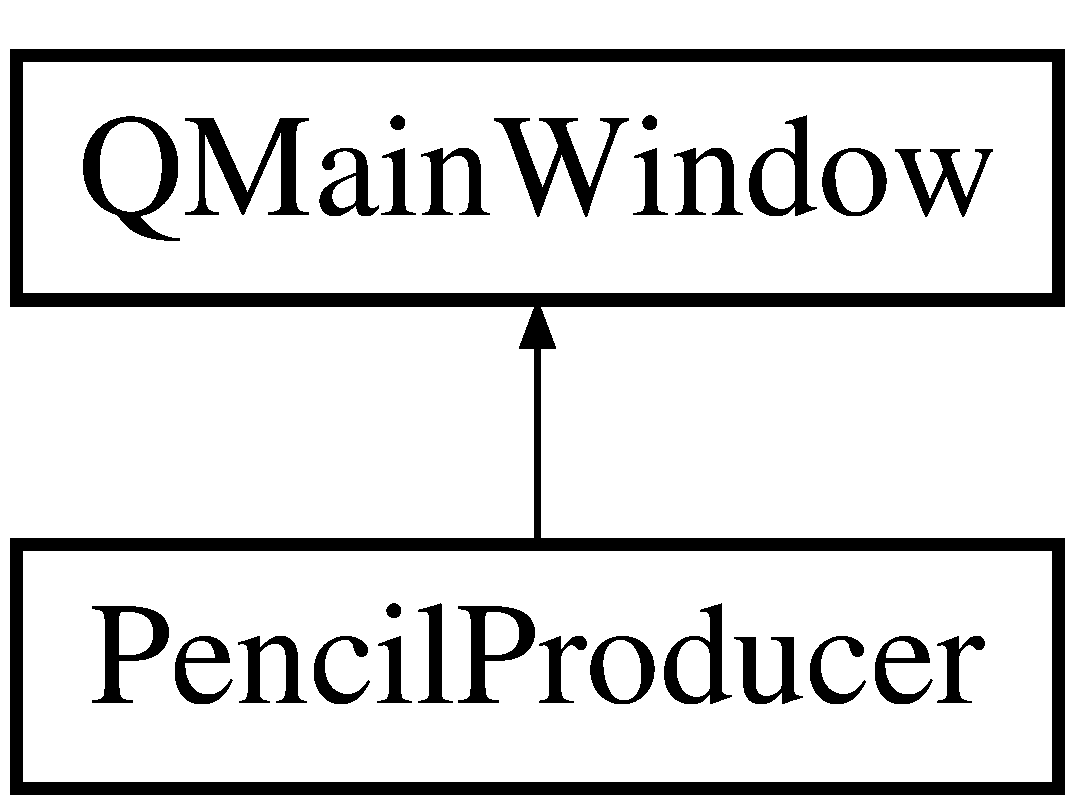
\includegraphics[height=2.000000cm]{classPencilProducer}
\end{center}
\end{figure}
\subsection*{Public Member Functions}
\begin{DoxyCompactItemize}
\item 
\hyperlink{classPencilProducer_a7b5425cd4bfd41d7b9cc9fe04101df06}{Pencil\+Producer} (Q\+Widget $\ast$parent=nullptr)
\item 
\hyperlink{classPencilProducer_a6e4548750600eb7b6886538a23ba4808}{$\sim$\+Pencil\+Producer} ()
\end{DoxyCompactItemize}
\subsection*{Private Slots}
\begin{DoxyCompactItemize}
\item 
void \hyperlink{classPencilProducer_a4463cb3676d728734fb935c8ea6fcb14}{on\+\_\+minus\+\_\+clicked} ()
\item 
void \hyperlink{classPencilProducer_a4f25cb44f7656627fb2118db163c6294}{on\+\_\+plus\+\_\+clicked} ()
\item 
void \hyperlink{classPencilProducer_a349d36fe7bfb716010b7ee0172e2ba88}{on\+\_\+buy\+Wood\+\_\+clicked} ()
\item 
void \hyperlink{classPencilProducer_aa6d6a98ad6b815634efbbf263605824e}{on\+\_\+buy\+Graphite\+\_\+clicked} ()
\item 
void \hyperlink{classPencilProducer_a9a278b633e203bc16941093ca1727c85}{on\+\_\+make\+Pencil\+\_\+clicked} ()
\item 
void \hyperlink{classPencilProducer_a2d54ee1f50fa095221bde3adf0d71d95}{on\+\_\+buy\+More\+\_\+clicked} ()
\item 
void \hyperlink{classPencilProducer_af182bfe6656f6e068da6feb74afa0bec}{update\+All} ()
\end{DoxyCompactItemize}
\subsection*{Private Member Functions}
\begin{DoxyCompactItemize}
\item 
void \hyperlink{classPencilProducer_afcd36c151c55ad1c9024873050eaee4d}{update} ()
\begin{DoxyCompactList}\small\item\em \hyperlink{classPencilProducer_afcd36c151c55ad1c9024873050eaee4d}{Pencil\+Producer\+::update} updates all values displayed on the UI and. \end{DoxyCompactList}\item 
void \hyperlink{classPencilProducer_ae4a56a7023ae3bb0b3f781c3f2a99d7e}{start\+Timer} ()
\end{DoxyCompactItemize}
\subsection*{Private Attributes}
\begin{DoxyCompactItemize}
\item 
Ui\+::\+Pencil\+Producer $\ast$ \hyperlink{classPencilProducer_af8ef000b90959052d1ab135ca9764621}{ui}
\item 
\hyperlink{classWallet}{Wallet} \hyperlink{classPencilProducer_a9ce8a9dbf5deb875692d5dcec4374e2d}{wallet}
\item 
\hyperlink{classGraphite__Inventory}{Graphite\+\_\+\+Inventory} \hyperlink{classPencilProducer_a04a8078a404418407a30a4175aaf890a}{graphite\+Inventory}
\item 
\hyperlink{classWood__Inventory}{Wood\+\_\+\+Inventory} \hyperlink{classPencilProducer_ac0454fe420705b3e3e922661e89ecee0}{wood\+Inventory}
\item 
\hyperlink{classPencil__Inventory}{Pencil\+\_\+\+Inventory} \hyperlink{classPencilProducer_ad1c13392410c1e57b6baff0bfde51e75}{pencil\+Inventory}
\item 
\hyperlink{classAPM2000__Inventory}{A\+P\+M2000\+\_\+\+Inventory} \hyperlink{classPencilProducer_a6af6334d9d18c19f235411a4c5fafb46}{apm2000\+Inventory}
\end{DoxyCompactItemize}


\subsection{Detailed Description}
Class to implement the Pencil Producer game  In this class we will define the constructor/descructor and all the other methods we need to make it run. As for the first Spring, we are in need of a cons/dest only. 

\subsection{Constructor \& Destructor Documentation}
\mbox{\Hypertarget{classPencilProducer_a7b5425cd4bfd41d7b9cc9fe04101df06}\label{classPencilProducer_a7b5425cd4bfd41d7b9cc9fe04101df06}} 
\index{Pencil\+Producer@{Pencil\+Producer}!Pencil\+Producer@{Pencil\+Producer}}
\index{Pencil\+Producer@{Pencil\+Producer}!Pencil\+Producer@{Pencil\+Producer}}
\subsubsection{\texorpdfstring{Pencil\+Producer()}{PencilProducer()}}
{\footnotesize\ttfamily Pencil\+Producer\+::\+Pencil\+Producer (\begin{DoxyParamCaption}\item[{Q\+Widget $\ast$}]{parent = {\ttfamily nullptr} }\end{DoxyParamCaption})\hspace{0.3cm}{\ttfamily [explicit]}}

Default constructor. \mbox{\Hypertarget{classPencilProducer_a6e4548750600eb7b6886538a23ba4808}\label{classPencilProducer_a6e4548750600eb7b6886538a23ba4808}} 
\index{Pencil\+Producer@{Pencil\+Producer}!````~Pencil\+Producer@{$\sim$\+Pencil\+Producer}}
\index{````~Pencil\+Producer@{$\sim$\+Pencil\+Producer}!Pencil\+Producer@{Pencil\+Producer}}
\subsubsection{\texorpdfstring{$\sim$\+Pencil\+Producer()}{~PencilProducer()}}
{\footnotesize\ttfamily Pencil\+Producer\+::$\sim$\+Pencil\+Producer (\begin{DoxyParamCaption}{ }\end{DoxyParamCaption})}

Default desctructor. 

\subsection{Member Function Documentation}
\mbox{\Hypertarget{classPencilProducer_aa6d6a98ad6b815634efbbf263605824e}\label{classPencilProducer_aa6d6a98ad6b815634efbbf263605824e}} 
\index{Pencil\+Producer@{Pencil\+Producer}!on\+\_\+buy\+Graphite\+\_\+clicked@{on\+\_\+buy\+Graphite\+\_\+clicked}}
\index{on\+\_\+buy\+Graphite\+\_\+clicked@{on\+\_\+buy\+Graphite\+\_\+clicked}!Pencil\+Producer@{Pencil\+Producer}}
\subsubsection{\texorpdfstring{on\+\_\+buy\+Graphite\+\_\+clicked}{on\_buyGraphite\_clicked}}
{\footnotesize\ttfamily void Pencil\+Producer\+::on\+\_\+buy\+Graphite\+\_\+clicked (\begin{DoxyParamCaption}{ }\end{DoxyParamCaption})\hspace{0.3cm}{\ttfamily [private]}, {\ttfamily [slot]}}

\mbox{\Hypertarget{classPencilProducer_a2d54ee1f50fa095221bde3adf0d71d95}\label{classPencilProducer_a2d54ee1f50fa095221bde3adf0d71d95}} 
\index{Pencil\+Producer@{Pencil\+Producer}!on\+\_\+buy\+More\+\_\+clicked@{on\+\_\+buy\+More\+\_\+clicked}}
\index{on\+\_\+buy\+More\+\_\+clicked@{on\+\_\+buy\+More\+\_\+clicked}!Pencil\+Producer@{Pencil\+Producer}}
\subsubsection{\texorpdfstring{on\+\_\+buy\+More\+\_\+clicked}{on\_buyMore\_clicked}}
{\footnotesize\ttfamily void Pencil\+Producer\+::on\+\_\+buy\+More\+\_\+clicked (\begin{DoxyParamCaption}{ }\end{DoxyParamCaption})\hspace{0.3cm}{\ttfamily [private]}, {\ttfamily [slot]}}

\mbox{\Hypertarget{classPencilProducer_a349d36fe7bfb716010b7ee0172e2ba88}\label{classPencilProducer_a349d36fe7bfb716010b7ee0172e2ba88}} 
\index{Pencil\+Producer@{Pencil\+Producer}!on\+\_\+buy\+Wood\+\_\+clicked@{on\+\_\+buy\+Wood\+\_\+clicked}}
\index{on\+\_\+buy\+Wood\+\_\+clicked@{on\+\_\+buy\+Wood\+\_\+clicked}!Pencil\+Producer@{Pencil\+Producer}}
\subsubsection{\texorpdfstring{on\+\_\+buy\+Wood\+\_\+clicked}{on\_buyWood\_clicked}}
{\footnotesize\ttfamily void Pencil\+Producer\+::on\+\_\+buy\+Wood\+\_\+clicked (\begin{DoxyParamCaption}{ }\end{DoxyParamCaption})\hspace{0.3cm}{\ttfamily [private]}, {\ttfamily [slot]}}

\mbox{\Hypertarget{classPencilProducer_a9a278b633e203bc16941093ca1727c85}\label{classPencilProducer_a9a278b633e203bc16941093ca1727c85}} 
\index{Pencil\+Producer@{Pencil\+Producer}!on\+\_\+make\+Pencil\+\_\+clicked@{on\+\_\+make\+Pencil\+\_\+clicked}}
\index{on\+\_\+make\+Pencil\+\_\+clicked@{on\+\_\+make\+Pencil\+\_\+clicked}!Pencil\+Producer@{Pencil\+Producer}}
\subsubsection{\texorpdfstring{on\+\_\+make\+Pencil\+\_\+clicked}{on\_makePencil\_clicked}}
{\footnotesize\ttfamily void Pencil\+Producer\+::on\+\_\+make\+Pencil\+\_\+clicked (\begin{DoxyParamCaption}{ }\end{DoxyParamCaption})\hspace{0.3cm}{\ttfamily [private]}, {\ttfamily [slot]}}

\mbox{\Hypertarget{classPencilProducer_a4463cb3676d728734fb935c8ea6fcb14}\label{classPencilProducer_a4463cb3676d728734fb935c8ea6fcb14}} 
\index{Pencil\+Producer@{Pencil\+Producer}!on\+\_\+minus\+\_\+clicked@{on\+\_\+minus\+\_\+clicked}}
\index{on\+\_\+minus\+\_\+clicked@{on\+\_\+minus\+\_\+clicked}!Pencil\+Producer@{Pencil\+Producer}}
\subsubsection{\texorpdfstring{on\+\_\+minus\+\_\+clicked}{on\_minus\_clicked}}
{\footnotesize\ttfamily void Pencil\+Producer\+::on\+\_\+minus\+\_\+clicked (\begin{DoxyParamCaption}{ }\end{DoxyParamCaption})\hspace{0.3cm}{\ttfamily [private]}, {\ttfamily [slot]}}

\mbox{\Hypertarget{classPencilProducer_a4f25cb44f7656627fb2118db163c6294}\label{classPencilProducer_a4f25cb44f7656627fb2118db163c6294}} 
\index{Pencil\+Producer@{Pencil\+Producer}!on\+\_\+plus\+\_\+clicked@{on\+\_\+plus\+\_\+clicked}}
\index{on\+\_\+plus\+\_\+clicked@{on\+\_\+plus\+\_\+clicked}!Pencil\+Producer@{Pencil\+Producer}}
\subsubsection{\texorpdfstring{on\+\_\+plus\+\_\+clicked}{on\_plus\_clicked}}
{\footnotesize\ttfamily void Pencil\+Producer\+::on\+\_\+plus\+\_\+clicked (\begin{DoxyParamCaption}{ }\end{DoxyParamCaption})\hspace{0.3cm}{\ttfamily [private]}, {\ttfamily [slot]}}

\mbox{\Hypertarget{classPencilProducer_ae4a56a7023ae3bb0b3f781c3f2a99d7e}\label{classPencilProducer_ae4a56a7023ae3bb0b3f781c3f2a99d7e}} 
\index{Pencil\+Producer@{Pencil\+Producer}!start\+Timer@{start\+Timer}}
\index{start\+Timer@{start\+Timer}!Pencil\+Producer@{Pencil\+Producer}}
\subsubsection{\texorpdfstring{start\+Timer()}{startTimer()}}
{\footnotesize\ttfamily void Pencil\+Producer\+::start\+Timer (\begin{DoxyParamCaption}{ }\end{DoxyParamCaption})\hspace{0.3cm}{\ttfamily [private]}}

\mbox{\Hypertarget{classPencilProducer_afcd36c151c55ad1c9024873050eaee4d}\label{classPencilProducer_afcd36c151c55ad1c9024873050eaee4d}} 
\index{Pencil\+Producer@{Pencil\+Producer}!update@{update}}
\index{update@{update}!Pencil\+Producer@{Pencil\+Producer}}
\subsubsection{\texorpdfstring{update()}{update()}}
{\footnotesize\ttfamily void Pencil\+Producer\+::update (\begin{DoxyParamCaption}{ }\end{DoxyParamCaption})\hspace{0.3cm}{\ttfamily [private]}}



\hyperlink{classPencilProducer_afcd36c151c55ad1c9024873050eaee4d}{Pencil\+Producer\+::update} updates all values displayed on the UI and. 

\mbox{\Hypertarget{classPencilProducer_af182bfe6656f6e068da6feb74afa0bec}\label{classPencilProducer_af182bfe6656f6e068da6feb74afa0bec}} 
\index{Pencil\+Producer@{Pencil\+Producer}!update\+All@{update\+All}}
\index{update\+All@{update\+All}!Pencil\+Producer@{Pencil\+Producer}}
\subsubsection{\texorpdfstring{update\+All}{updateAll}}
{\footnotesize\ttfamily void Pencil\+Producer\+::update\+All (\begin{DoxyParamCaption}{ }\end{DoxyParamCaption})\hspace{0.3cm}{\ttfamily [private]}, {\ttfamily [slot]}}



\subsection{Member Data Documentation}
\mbox{\Hypertarget{classPencilProducer_a6af6334d9d18c19f235411a4c5fafb46}\label{classPencilProducer_a6af6334d9d18c19f235411a4c5fafb46}} 
\index{Pencil\+Producer@{Pencil\+Producer}!apm2000\+Inventory@{apm2000\+Inventory}}
\index{apm2000\+Inventory@{apm2000\+Inventory}!Pencil\+Producer@{Pencil\+Producer}}
\subsubsection{\texorpdfstring{apm2000\+Inventory}{apm2000Inventory}}
{\footnotesize\ttfamily \hyperlink{classAPM2000__Inventory}{A\+P\+M2000\+\_\+\+Inventory} Pencil\+Producer\+::apm2000\+Inventory\hspace{0.3cm}{\ttfamily [private]}}

\mbox{\Hypertarget{classPencilProducer_a04a8078a404418407a30a4175aaf890a}\label{classPencilProducer_a04a8078a404418407a30a4175aaf890a}} 
\index{Pencil\+Producer@{Pencil\+Producer}!graphite\+Inventory@{graphite\+Inventory}}
\index{graphite\+Inventory@{graphite\+Inventory}!Pencil\+Producer@{Pencil\+Producer}}
\subsubsection{\texorpdfstring{graphite\+Inventory}{graphiteInventory}}
{\footnotesize\ttfamily \hyperlink{classGraphite__Inventory}{Graphite\+\_\+\+Inventory} Pencil\+Producer\+::graphite\+Inventory\hspace{0.3cm}{\ttfamily [private]}}

\mbox{\Hypertarget{classPencilProducer_ad1c13392410c1e57b6baff0bfde51e75}\label{classPencilProducer_ad1c13392410c1e57b6baff0bfde51e75}} 
\index{Pencil\+Producer@{Pencil\+Producer}!pencil\+Inventory@{pencil\+Inventory}}
\index{pencil\+Inventory@{pencil\+Inventory}!Pencil\+Producer@{Pencil\+Producer}}
\subsubsection{\texorpdfstring{pencil\+Inventory}{pencilInventory}}
{\footnotesize\ttfamily \hyperlink{classPencil__Inventory}{Pencil\+\_\+\+Inventory} Pencil\+Producer\+::pencil\+Inventory\hspace{0.3cm}{\ttfamily [private]}}

\mbox{\Hypertarget{classPencilProducer_af8ef000b90959052d1ab135ca9764621}\label{classPencilProducer_af8ef000b90959052d1ab135ca9764621}} 
\index{Pencil\+Producer@{Pencil\+Producer}!ui@{ui}}
\index{ui@{ui}!Pencil\+Producer@{Pencil\+Producer}}
\subsubsection{\texorpdfstring{ui}{ui}}
{\footnotesize\ttfamily Ui\+::\+Pencil\+Producer$\ast$ Pencil\+Producer\+::ui\hspace{0.3cm}{\ttfamily [private]}}

Create the UI widget for the window \mbox{\Hypertarget{classPencilProducer_a9ce8a9dbf5deb875692d5dcec4374e2d}\label{classPencilProducer_a9ce8a9dbf5deb875692d5dcec4374e2d}} 
\index{Pencil\+Producer@{Pencil\+Producer}!wallet@{wallet}}
\index{wallet@{wallet}!Pencil\+Producer@{Pencil\+Producer}}
\subsubsection{\texorpdfstring{wallet}{wallet}}
{\footnotesize\ttfamily \hyperlink{classWallet}{Wallet} Pencil\+Producer\+::wallet\hspace{0.3cm}{\ttfamily [private]}}

\mbox{\Hypertarget{classPencilProducer_ac0454fe420705b3e3e922661e89ecee0}\label{classPencilProducer_ac0454fe420705b3e3e922661e89ecee0}} 
\index{Pencil\+Producer@{Pencil\+Producer}!wood\+Inventory@{wood\+Inventory}}
\index{wood\+Inventory@{wood\+Inventory}!Pencil\+Producer@{Pencil\+Producer}}
\subsubsection{\texorpdfstring{wood\+Inventory}{woodInventory}}
{\footnotesize\ttfamily \hyperlink{classWood__Inventory}{Wood\+\_\+\+Inventory} Pencil\+Producer\+::wood\+Inventory\hspace{0.3cm}{\ttfamily [private]}}



The documentation for this class was generated from the following files\+:\begin{DoxyCompactItemize}
\item 
/mnt/0896595996594878/\+Users/\+Maverick/\+Documents/\+University/\+School/\+Modules/4th Semester/\+Applied Computer Science/\+Software Eng/\+Project/\+Sprint\+\_\+02/se-\/02-\/team-\/09/\+Pencil-\/\+Producer/\hyperlink{pencilproducer_8h}{pencilproducer.\+h}\item 
/mnt/0896595996594878/\+Users/\+Maverick/\+Documents/\+University/\+School/\+Modules/4th Semester/\+Applied Computer Science/\+Software Eng/\+Project/\+Sprint\+\_\+02/se-\/02-\/team-\/09/\+Pencil-\/\+Producer/\hyperlink{pencilproducer_8cpp}{pencilproducer.\+cpp}\end{DoxyCompactItemize}

\hypertarget{classWallet}{}\section{Wallet Class Reference}
\label{classWallet}\index{Wallet@{Wallet}}


The \hyperlink{classWallet}{Wallet} class keeps track of bank balance and methods for crediting/debiting account.  




{\ttfamily \#include $<$wallet.\+h$>$}

\subsection*{Public Member Functions}
\begin{DoxyCompactItemize}
\item 
\hyperlink{classWallet_ad9be9e49244b78db9099fcaeccd1af04}{Wallet} ()
\begin{DoxyCompactList}\small\item\em \hyperlink{classWallet_ad9be9e49244b78db9099fcaeccd1af04}{Wallet\+::\+Wallet} wallet constructor. Default balance \$145.\+00. \end{DoxyCompactList}\item 
float \hyperlink{classWallet_a92536035a1de76dc7842693beb93cd24}{get\+Bank\+Balance} () const
\begin{DoxyCompactList}\small\item\em \hyperlink{classWallet_a92536035a1de76dc7842693beb93cd24}{Wallet\+::get\+Bank\+Balance}. \end{DoxyCompactList}\item 
void \hyperlink{classWallet_ab9354b0a8250c0f21b867cc725a33e1e}{credit\+Money} (float)
\begin{DoxyCompactList}\small\item\em \hyperlink{classWallet_ab9354b0a8250c0f21b867cc725a33e1e}{Wallet\+::credit\+Money} credits bank balance. \end{DoxyCompactList}\item 
void \hyperlink{classWallet_a8be722d227a610e4b36b79c2eb04c73f}{debit\+Money} (float)
\begin{DoxyCompactList}\small\item\em \hyperlink{classWallet_a8be722d227a610e4b36b79c2eb04c73f}{Wallet\+::debit\+Money} debits bank balance. \end{DoxyCompactList}\item 
bool \hyperlink{classWallet_a69b488bc31201592bb860b6fdaafa1b8}{can\+Credit\+Money} (float) const
\begin{DoxyCompactList}\small\item\em \hyperlink{classWallet_a69b488bc31201592bb860b6fdaafa1b8}{Wallet\+::can\+Credit\+Money}. \end{DoxyCompactList}\item 
bool \hyperlink{classWallet_a1583a38c87dd04ecd5854f15590e170d}{can\+Debit\+Money} (float) const
\begin{DoxyCompactList}\small\item\em \hyperlink{classWallet_a1583a38c87dd04ecd5854f15590e170d}{Wallet\+::can\+Debit\+Money}. \end{DoxyCompactList}\end{DoxyCompactItemize}
\subsection*{Private Attributes}
\begin{DoxyCompactItemize}
\item 
float \hyperlink{classWallet_a586fc4e3fb0e9ce59e5bbafd9145d319}{bank\+Balance}
\begin{DoxyCompactList}\small\item\em bank balance. Default value set to \$145.\+00 \end{DoxyCompactList}\end{DoxyCompactItemize}


\subsection{Detailed Description}
The \hyperlink{classWallet}{Wallet} class keeps track of bank balance and methods for crediting/debiting account. 

\subsection{Constructor \& Destructor Documentation}
\mbox{\Hypertarget{classWallet_ad9be9e49244b78db9099fcaeccd1af04}\label{classWallet_ad9be9e49244b78db9099fcaeccd1af04}} 
\index{Wallet@{Wallet}!Wallet@{Wallet}}
\index{Wallet@{Wallet}!Wallet@{Wallet}}
\subsubsection{\texorpdfstring{Wallet()}{Wallet()}}
{\footnotesize\ttfamily Wallet\+::\+Wallet (\begin{DoxyParamCaption}{ }\end{DoxyParamCaption})}



\hyperlink{classWallet_ad9be9e49244b78db9099fcaeccd1af04}{Wallet\+::\+Wallet} wallet constructor. Default balance \$145.\+00. 



\subsection{Member Function Documentation}
\mbox{\Hypertarget{classWallet_a69b488bc31201592bb860b6fdaafa1b8}\label{classWallet_a69b488bc31201592bb860b6fdaafa1b8}} 
\index{Wallet@{Wallet}!can\+Credit\+Money@{can\+Credit\+Money}}
\index{can\+Credit\+Money@{can\+Credit\+Money}!Wallet@{Wallet}}
\subsubsection{\texorpdfstring{can\+Credit\+Money()}{canCreditMoney()}}
{\footnotesize\ttfamily bool Wallet\+::can\+Credit\+Money (\begin{DoxyParamCaption}\item[{float}]{money }\end{DoxyParamCaption}) const}



\hyperlink{classWallet_a69b488bc31201592bb860b6fdaafa1b8}{Wallet\+::can\+Credit\+Money}. 


\begin{DoxyParams}{Parameters}
{\em money} & amount to credit \\
\hline
\end{DoxyParams}
\begin{DoxyReturn}{Returns}
true if amount to credit is positive, false otherwise 
\end{DoxyReturn}
\mbox{\Hypertarget{classWallet_a1583a38c87dd04ecd5854f15590e170d}\label{classWallet_a1583a38c87dd04ecd5854f15590e170d}} 
\index{Wallet@{Wallet}!can\+Debit\+Money@{can\+Debit\+Money}}
\index{can\+Debit\+Money@{can\+Debit\+Money}!Wallet@{Wallet}}
\subsubsection{\texorpdfstring{can\+Debit\+Money()}{canDebitMoney()}}
{\footnotesize\ttfamily bool Wallet\+::can\+Debit\+Money (\begin{DoxyParamCaption}\item[{float}]{money }\end{DoxyParamCaption}) const}



\hyperlink{classWallet_a1583a38c87dd04ecd5854f15590e170d}{Wallet\+::can\+Debit\+Money}. 


\begin{DoxyParams}{Parameters}
{\em money} & amount to debit \\
\hline
\end{DoxyParams}
\begin{DoxyReturn}{Returns}
true if amount to debit is not greater than bank balance and amount to debit is positive, false otherwise 
\end{DoxyReturn}
\mbox{\Hypertarget{classWallet_ab9354b0a8250c0f21b867cc725a33e1e}\label{classWallet_ab9354b0a8250c0f21b867cc725a33e1e}} 
\index{Wallet@{Wallet}!credit\+Money@{credit\+Money}}
\index{credit\+Money@{credit\+Money}!Wallet@{Wallet}}
\subsubsection{\texorpdfstring{credit\+Money()}{creditMoney()}}
{\footnotesize\ttfamily void Wallet\+::credit\+Money (\begin{DoxyParamCaption}\item[{float}]{money }\end{DoxyParamCaption})}



\hyperlink{classWallet_ab9354b0a8250c0f21b867cc725a33e1e}{Wallet\+::credit\+Money} credits bank balance. 


\begin{DoxyParams}{Parameters}
{\em money} & amount to credit bank balance \\
\hline
\end{DoxyParams}
\mbox{\Hypertarget{classWallet_a8be722d227a610e4b36b79c2eb04c73f}\label{classWallet_a8be722d227a610e4b36b79c2eb04c73f}} 
\index{Wallet@{Wallet}!debit\+Money@{debit\+Money}}
\index{debit\+Money@{debit\+Money}!Wallet@{Wallet}}
\subsubsection{\texorpdfstring{debit\+Money()}{debitMoney()}}
{\footnotesize\ttfamily void Wallet\+::debit\+Money (\begin{DoxyParamCaption}\item[{float}]{money }\end{DoxyParamCaption})}



\hyperlink{classWallet_a8be722d227a610e4b36b79c2eb04c73f}{Wallet\+::debit\+Money} debits bank balance. 


\begin{DoxyParams}{Parameters}
{\em money} & amount to debit bank balance \\
\hline
\end{DoxyParams}
\mbox{\Hypertarget{classWallet_a92536035a1de76dc7842693beb93cd24}\label{classWallet_a92536035a1de76dc7842693beb93cd24}} 
\index{Wallet@{Wallet}!get\+Bank\+Balance@{get\+Bank\+Balance}}
\index{get\+Bank\+Balance@{get\+Bank\+Balance}!Wallet@{Wallet}}
\subsubsection{\texorpdfstring{get\+Bank\+Balance()}{getBankBalance()}}
{\footnotesize\ttfamily float Wallet\+::get\+Bank\+Balance (\begin{DoxyParamCaption}{ }\end{DoxyParamCaption}) const}



\hyperlink{classWallet_a92536035a1de76dc7842693beb93cd24}{Wallet\+::get\+Bank\+Balance}. 

\begin{DoxyReturn}{Returns}
float bank\+Balance 
\end{DoxyReturn}


\subsection{Member Data Documentation}
\mbox{\Hypertarget{classWallet_a586fc4e3fb0e9ce59e5bbafd9145d319}\label{classWallet_a586fc4e3fb0e9ce59e5bbafd9145d319}} 
\index{Wallet@{Wallet}!bank\+Balance@{bank\+Balance}}
\index{bank\+Balance@{bank\+Balance}!Wallet@{Wallet}}
\subsubsection{\texorpdfstring{bank\+Balance}{bankBalance}}
{\footnotesize\ttfamily float Wallet\+::bank\+Balance\hspace{0.3cm}{\ttfamily [private]}}



bank balance. Default value set to \$145.\+00 



The documentation for this class was generated from the following files\+:\begin{DoxyCompactItemize}
\item 
/mnt/0896595996594878/\+Users/\+Maverick/\+Documents/\+University/\+School/\+Modules/4th Semester/\+Applied Computer Science/\+Software Eng/\+Project/\+Sprint\+\_\+02/se-\/02-\/team-\/09/\+Pencil-\/\+Producer/\hyperlink{wallet_8h}{wallet.\+h}\item 
/mnt/0896595996594878/\+Users/\+Maverick/\+Documents/\+University/\+School/\+Modules/4th Semester/\+Applied Computer Science/\+Software Eng/\+Project/\+Sprint\+\_\+02/se-\/02-\/team-\/09/\+Pencil-\/\+Producer/\hyperlink{wallet_8cpp}{wallet.\+cpp}\end{DoxyCompactItemize}

\hypertarget{classWood__Inventory}{}\section{Wood\+\_\+\+Inventory Class Reference}
\label{classWood__Inventory}\index{Wood\+\_\+\+Inventory@{Wood\+\_\+\+Inventory}}


{\ttfamily \#include $<$wood\+\_\+inventory.\+h$>$}

Inheritance diagram for Wood\+\_\+\+Inventory\+:\begin{figure}[H]
\begin{center}
\leavevmode
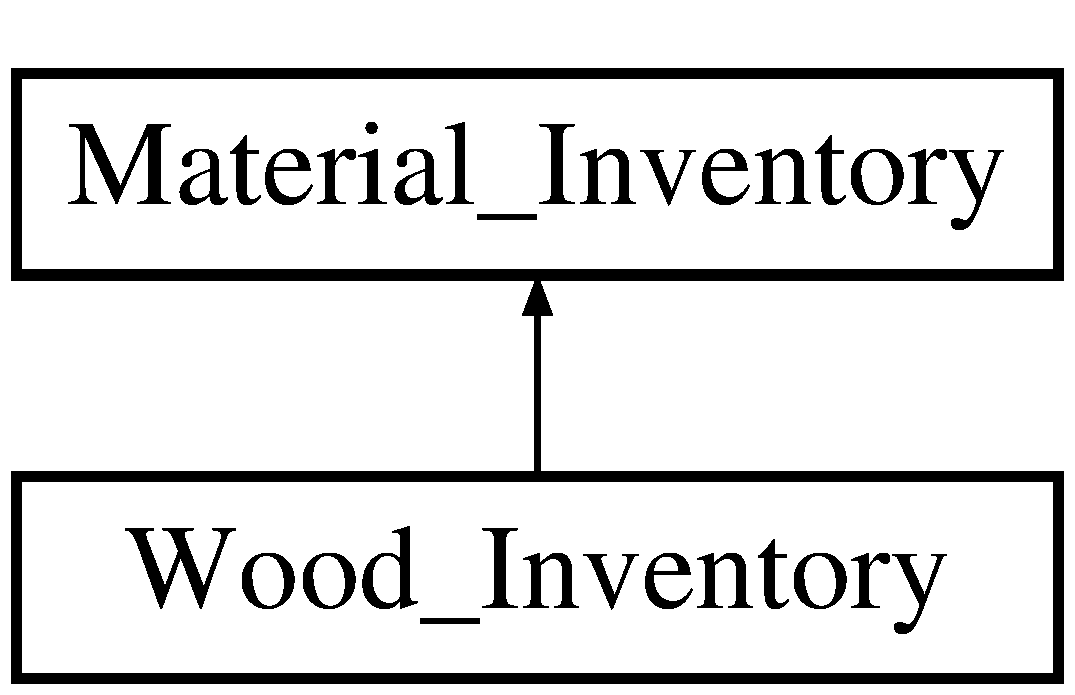
\includegraphics[height=2.000000cm]{classWood__Inventory}
\end{center}
\end{figure}
\subsection*{Public Member Functions}
\begin{DoxyCompactItemize}
\item 
\hyperlink{classWood__Inventory_afcf1c5469106083ce0ab7a7ee5e15523}{Wood\+\_\+\+Inventory} ()
\end{DoxyCompactItemize}


\subsection{Constructor \& Destructor Documentation}
\mbox{\Hypertarget{classWood__Inventory_afcf1c5469106083ce0ab7a7ee5e15523}\label{classWood__Inventory_afcf1c5469106083ce0ab7a7ee5e15523}} 
\index{Wood\+\_\+\+Inventory@{Wood\+\_\+\+Inventory}!Wood\+\_\+\+Inventory@{Wood\+\_\+\+Inventory}}
\index{Wood\+\_\+\+Inventory@{Wood\+\_\+\+Inventory}!Wood\+\_\+\+Inventory@{Wood\+\_\+\+Inventory}}
\subsubsection{\texorpdfstring{Wood\+\_\+\+Inventory()}{Wood\_Inventory()}}
{\footnotesize\ttfamily Wood\+\_\+\+Inventory\+::\+Wood\+\_\+\+Inventory (\begin{DoxyParamCaption}{ }\end{DoxyParamCaption})}



The documentation for this class was generated from the following files\+:\begin{DoxyCompactItemize}
\item 
/mnt/0896595996594878/\+Users/\+Maverick/\+Documents/\+University/\+School/\+Modules/4th Semester/\+Applied Computer Science/\+Software Eng/\+Project/\+Sprint\+\_\+02/se-\/02-\/team-\/09/\+Pencil-\/\+Producer/\hyperlink{wood__inventory_8h}{wood\+\_\+inventory.\+h}\item 
/mnt/0896595996594878/\+Users/\+Maverick/\+Documents/\+University/\+School/\+Modules/4th Semester/\+Applied Computer Science/\+Software Eng/\+Project/\+Sprint\+\_\+02/se-\/02-\/team-\/09/\+Pencil-\/\+Producer/\hyperlink{wood__inventory_8cpp}{wood\+\_\+inventory.\+cpp}\end{DoxyCompactItemize}

\chapter{File Documentation}
\hypertarget{apm2000__inventory_8cpp}{}\section{/mnt/0896595996594878/\+Users/\+Maverick/\+Documents/\+University/\+School/\+Modules/4th Semester/\+Applied Computer Science/\+Software Eng/\+Project/\+Sprint\+\_\+02/se-\/02-\/team-\/09/\+Pencil-\/\+Producer/apm2000\+\_\+inventory.cpp File Reference}
\label{apm2000__inventory_8cpp}\index{/mnt/0896595996594878/\+Users/\+Maverick/\+Documents/\+University/\+School/\+Modules/4th Semester/\+Applied Computer Science/\+Software Eng/\+Project/\+Sprint\+\_\+02/se-\/02-\/team-\/09/\+Pencil-\/\+Producer/apm2000\+\_\+inventory.\+cpp@{/mnt/0896595996594878/\+Users/\+Maverick/\+Documents/\+University/\+School/\+Modules/4th Semester/\+Applied Computer Science/\+Software Eng/\+Project/\+Sprint\+\_\+02/se-\/02-\/team-\/09/\+Pencil-\/\+Producer/apm2000\+\_\+inventory.\+cpp}}
{\ttfamily \#include \char`\"{}apm2000\+\_\+inventory.\+h\char`\"{}}\newline

\hypertarget{apm2000__inventory_8h}{}\section{/mnt/0896595996594878/\+Users/\+Maverick/\+Documents/\+University/\+School/\+Modules/4th Semester/\+Applied Computer Science/\+Software Eng/\+Project/\+Sprint\+\_\+02/se-\/02-\/team-\/09/\+Pencil-\/\+Producer/apm2000\+\_\+inventory.h File Reference}
\label{apm2000__inventory_8h}\index{/mnt/0896595996594878/\+Users/\+Maverick/\+Documents/\+University/\+School/\+Modules/4th Semester/\+Applied Computer Science/\+Software Eng/\+Project/\+Sprint\+\_\+02/se-\/02-\/team-\/09/\+Pencil-\/\+Producer/apm2000\+\_\+inventory.\+h@{/mnt/0896595996594878/\+Users/\+Maverick/\+Documents/\+University/\+School/\+Modules/4th Semester/\+Applied Computer Science/\+Software Eng/\+Project/\+Sprint\+\_\+02/se-\/02-\/team-\/09/\+Pencil-\/\+Producer/apm2000\+\_\+inventory.\+h}}
{\ttfamily \#include \char`\"{}wallet.\+h\char`\"{}}\newline
{\ttfamily \#include \char`\"{}pencil\+\_\+inventory.\+h\char`\"{}}\newline
{\ttfamily \#include \char`\"{}graphite\+\_\+inventory.\+h\char`\"{}}\newline
{\ttfamily \#include \char`\"{}wood\+\_\+inventory.\+h\char`\"{}}\newline
\subsection*{Classes}
\begin{DoxyCompactItemize}
\item 
class \hyperlink{classAPM2000__Inventory}{A\+P\+M2000\+\_\+\+Inventory}
\begin{DoxyCompactList}\small\item\em The \hyperlink{classAPM2000__Inventory}{A\+P\+M2000\+\_\+\+Inventory} class Automatic Pencil Machine(\+A\+P\+M)~\newline
Suffix \char`\"{}2000\char`\"{} indicates 2000-\/series. Every 2000-\/series produces 2 pencils per second, which are automatically added into the inventory. A\+PM stops automatically when there are insufficient materials and resumes when materials are available. \end{DoxyCompactList}\end{DoxyCompactItemize}

\hypertarget{graphite__inventory_8cpp}{}\section{/mnt/0896595996594878/\+Users/\+Maverick/\+Documents/\+University/\+School/\+Modules/4th Semester/\+Applied Computer Science/\+Software Eng/\+Project/\+Sprint\+\_\+02/se-\/02-\/team-\/09/\+Pencil-\/\+Producer/graphite\+\_\+inventory.cpp File Reference}
\label{graphite__inventory_8cpp}\index{/mnt/0896595996594878/\+Users/\+Maverick/\+Documents/\+University/\+School/\+Modules/4th Semester/\+Applied Computer Science/\+Software Eng/\+Project/\+Sprint\+\_\+02/se-\/02-\/team-\/09/\+Pencil-\/\+Producer/graphite\+\_\+inventory.\+cpp@{/mnt/0896595996594878/\+Users/\+Maverick/\+Documents/\+University/\+School/\+Modules/4th Semester/\+Applied Computer Science/\+Software Eng/\+Project/\+Sprint\+\_\+02/se-\/02-\/team-\/09/\+Pencil-\/\+Producer/graphite\+\_\+inventory.\+cpp}}
{\ttfamily \#include \char`\"{}graphite\+\_\+inventory.\+h\char`\"{}}\newline

\hypertarget{graphite__inventory_8h}{}\section{/mnt/0896595996594878/\+Users/\+Maverick/\+Documents/\+University/\+School/\+Modules/4th Semester/\+Applied Computer Science/\+Software Eng/\+Project/\+Sprint\+\_\+02/se-\/02-\/team-\/09/\+Pencil-\/\+Producer/graphite\+\_\+inventory.h File Reference}
\label{graphite__inventory_8h}\index{/mnt/0896595996594878/\+Users/\+Maverick/\+Documents/\+University/\+School/\+Modules/4th Semester/\+Applied Computer Science/\+Software Eng/\+Project/\+Sprint\+\_\+02/se-\/02-\/team-\/09/\+Pencil-\/\+Producer/graphite\+\_\+inventory.\+h@{/mnt/0896595996594878/\+Users/\+Maverick/\+Documents/\+University/\+School/\+Modules/4th Semester/\+Applied Computer Science/\+Software Eng/\+Project/\+Sprint\+\_\+02/se-\/02-\/team-\/09/\+Pencil-\/\+Producer/graphite\+\_\+inventory.\+h}}
{\ttfamily \#include \char`\"{}material\+\_\+inventory.\+h\char`\"{}}\newline
\subsection*{Classes}
\begin{DoxyCompactItemize}
\item 
class \hyperlink{classGraphite__Inventory}{Graphite\+\_\+\+Inventory}
\end{DoxyCompactItemize}

\hypertarget{main_8cpp}{}\section{/mnt/0896595996594878/\+Users/\+Maverick/\+Documents/\+University/\+School/\+Modules/4th Semester/\+Applied Computer Science/\+Software Eng/\+Project/\+Sprint\+\_\+02/se-\/02-\/team-\/09/\+Pencil-\/\+Producer/main.cpp File Reference}
\label{main_8cpp}\index{/mnt/0896595996594878/\+Users/\+Maverick/\+Documents/\+University/\+School/\+Modules/4th Semester/\+Applied Computer Science/\+Software Eng/\+Project/\+Sprint\+\_\+02/se-\/02-\/team-\/09/\+Pencil-\/\+Producer/main.\+cpp@{/mnt/0896595996594878/\+Users/\+Maverick/\+Documents/\+University/\+School/\+Modules/4th Semester/\+Applied Computer Science/\+Software Eng/\+Project/\+Sprint\+\_\+02/se-\/02-\/team-\/09/\+Pencil-\/\+Producer/main.\+cpp}}
{\ttfamily \#include \char`\"{}pencilproducer.\+h\char`\"{}}\newline
{\ttfamily \#include $<$Q\+Application$>$}\newline
\subsection*{Functions}
\begin{DoxyCompactItemize}
\item 
int \hyperlink{main_8cpp_a0ddf1224851353fc92bfbff6f499fa97}{main} (int argc, char $\ast$argv\mbox{[}$\,$\mbox{]})
\end{DoxyCompactItemize}


\subsection{Function Documentation}
\mbox{\Hypertarget{main_8cpp_a0ddf1224851353fc92bfbff6f499fa97}\label{main_8cpp_a0ddf1224851353fc92bfbff6f499fa97}} 
\index{main.\+cpp@{main.\+cpp}!main@{main}}
\index{main@{main}!main.\+cpp@{main.\+cpp}}
\subsubsection{\texorpdfstring{main()}{main()}}
{\footnotesize\ttfamily int main (\begin{DoxyParamCaption}\item[{int}]{argc,  }\item[{char $\ast$}]{argv\mbox{[}$\,$\mbox{]} }\end{DoxyParamCaption})}


\begin{DoxyParams}{Parameters}
{\em argc} & \\
\hline
{\em argv} & \\
\hline
\end{DoxyParams}
\begin{DoxyReturn}{Returns}
app.\+exec() 
\end{DoxyReturn}

\hypertarget{material__inventory_8cpp}{}\section{/mnt/0896595996594878/\+Users/\+Maverick/\+Documents/\+University/\+School/\+Modules/4th Semester/\+Applied Computer Science/\+Software Eng/\+Project/\+Sprint\+\_\+02/se-\/02-\/team-\/09/\+Pencil-\/\+Producer/material\+\_\+inventory.cpp File Reference}
\label{material__inventory_8cpp}\index{/mnt/0896595996594878/\+Users/\+Maverick/\+Documents/\+University/\+School/\+Modules/4th Semester/\+Applied Computer Science/\+Software Eng/\+Project/\+Sprint\+\_\+02/se-\/02-\/team-\/09/\+Pencil-\/\+Producer/material\+\_\+inventory.\+cpp@{/mnt/0896595996594878/\+Users/\+Maverick/\+Documents/\+University/\+School/\+Modules/4th Semester/\+Applied Computer Science/\+Software Eng/\+Project/\+Sprint\+\_\+02/se-\/02-\/team-\/09/\+Pencil-\/\+Producer/material\+\_\+inventory.\+cpp}}
{\ttfamily \#include \char`\"{}material\+\_\+inventory.\+h\char`\"{}}\newline

\hypertarget{material__inventory_8h}{}\section{/mnt/0896595996594878/\+Users/\+Maverick/\+Documents/\+University/\+School/\+Modules/4th Semester/\+Applied Computer Science/\+Software Eng/\+Project/\+Sprint\+\_\+02/se-\/02-\/team-\/09/\+Pencil-\/\+Producer/material\+\_\+inventory.h File Reference}
\label{material__inventory_8h}\index{/mnt/0896595996594878/\+Users/\+Maverick/\+Documents/\+University/\+School/\+Modules/4th Semester/\+Applied Computer Science/\+Software Eng/\+Project/\+Sprint\+\_\+02/se-\/02-\/team-\/09/\+Pencil-\/\+Producer/material\+\_\+inventory.\+h@{/mnt/0896595996594878/\+Users/\+Maverick/\+Documents/\+University/\+School/\+Modules/4th Semester/\+Applied Computer Science/\+Software Eng/\+Project/\+Sprint\+\_\+02/se-\/02-\/team-\/09/\+Pencil-\/\+Producer/material\+\_\+inventory.\+h}}
{\ttfamily \#include \char`\"{}wallet.\+h\char`\"{}}\newline
{\ttfamily \#include $<$cstdlib$>$}\newline
{\ttfamily \#include $<$ctime$>$}\newline
\subsection*{Classes}
\begin{DoxyCompactItemize}
\item 
class \hyperlink{classMaterial__Inventory}{Material\+\_\+\+Inventory}
\begin{DoxyCompactList}\small\item\em The \hyperlink{classMaterial__Inventory}{Material\+\_\+\+Inventory} class superclass of other material classes. \end{DoxyCompactList}\end{DoxyCompactItemize}

\hypertarget{pencil__inventory_8cpp}{}\section{/mnt/0896595996594878/\+Users/\+Maverick/\+Documents/\+University/\+School/\+Modules/4th Semester/\+Applied Computer Science/\+Software Eng/\+Project/\+Sprint\+\_\+02/se-\/02-\/team-\/09/\+Pencil-\/\+Producer/pencil\+\_\+inventory.cpp File Reference}
\label{pencil__inventory_8cpp}\index{/mnt/0896595996594878/\+Users/\+Maverick/\+Documents/\+University/\+School/\+Modules/4th Semester/\+Applied Computer Science/\+Software Eng/\+Project/\+Sprint\+\_\+02/se-\/02-\/team-\/09/\+Pencil-\/\+Producer/pencil\+\_\+inventory.\+cpp@{/mnt/0896595996594878/\+Users/\+Maverick/\+Documents/\+University/\+School/\+Modules/4th Semester/\+Applied Computer Science/\+Software Eng/\+Project/\+Sprint\+\_\+02/se-\/02-\/team-\/09/\+Pencil-\/\+Producer/pencil\+\_\+inventory.\+cpp}}
{\ttfamily \#include \char`\"{}pencil\+\_\+inventory.\+h\char`\"{}}\newline

\hypertarget{pencil__inventory_8h}{}\section{/mnt/0896595996594878/\+Users/\+Maverick/\+Documents/\+University/\+School/\+Modules/4th Semester/\+Applied Computer Science/\+Software Eng/\+Project/\+Sprint\+\_\+02/se-\/02-\/team-\/09/\+Pencil-\/\+Producer/pencil\+\_\+inventory.h File Reference}
\label{pencil__inventory_8h}\index{/mnt/0896595996594878/\+Users/\+Maverick/\+Documents/\+University/\+School/\+Modules/4th Semester/\+Applied Computer Science/\+Software Eng/\+Project/\+Sprint\+\_\+02/se-\/02-\/team-\/09/\+Pencil-\/\+Producer/pencil\+\_\+inventory.\+h@{/mnt/0896595996594878/\+Users/\+Maverick/\+Documents/\+University/\+School/\+Modules/4th Semester/\+Applied Computer Science/\+Software Eng/\+Project/\+Sprint\+\_\+02/se-\/02-\/team-\/09/\+Pencil-\/\+Producer/pencil\+\_\+inventory.\+h}}
{\ttfamily \#include \char`\"{}wallet.\+h\char`\"{}}\newline
{\ttfamily \#include \char`\"{}graphite\+\_\+inventory.\+h\char`\"{}}\newline
{\ttfamily \#include \char`\"{}wood\+\_\+inventory.\+h\char`\"{}}\newline
{\ttfamily \#include $<$cmath$>$}\newline
{\ttfamily \#include $<$iostream$>$}\newline
{\ttfamily \#include $<$algorithm$>$}\newline
\subsection*{Classes}
\begin{DoxyCompactItemize}
\item 
class \hyperlink{classPencil__Inventory}{Pencil\+\_\+\+Inventory}
\begin{DoxyCompactList}\small\item\em The \hyperlink{classPencil__Inventory}{Pencil\+\_\+\+Inventory} class main class for managing pencil prices and production. \end{DoxyCompactList}\end{DoxyCompactItemize}

\hypertarget{pencilproducer_8cpp}{}\section{/mnt/0896595996594878/\+Users/\+Maverick/\+Documents/\+University/\+School/\+Modules/4th Semester/\+Applied Computer Science/\+Software Eng/\+Project/\+Sprint\+\_\+02/se-\/02-\/team-\/09/\+Pencil-\/\+Producer/pencilproducer.cpp File Reference}
\label{pencilproducer_8cpp}\index{/mnt/0896595996594878/\+Users/\+Maverick/\+Documents/\+University/\+School/\+Modules/4th Semester/\+Applied Computer Science/\+Software Eng/\+Project/\+Sprint\+\_\+02/se-\/02-\/team-\/09/\+Pencil-\/\+Producer/pencilproducer.\+cpp@{/mnt/0896595996594878/\+Users/\+Maverick/\+Documents/\+University/\+School/\+Modules/4th Semester/\+Applied Computer Science/\+Software Eng/\+Project/\+Sprint\+\_\+02/se-\/02-\/team-\/09/\+Pencil-\/\+Producer/pencilproducer.\+cpp}}
{\ttfamily \#include \char`\"{}pencilproducer.\+h\char`\"{}}\newline
{\ttfamily \#include \char`\"{}ui\+\_\+pencilproducer.\+h\char`\"{}}\newline

\hypertarget{pencilproducer_8h}{}\section{/mnt/0896595996594878/\+Users/\+Maverick/\+Documents/\+University/\+School/\+Modules/4th Semester/\+Applied Computer Science/\+Software Eng/\+Project/\+Sprint\+\_\+02/se-\/02-\/team-\/09/\+Pencil-\/\+Producer/pencilproducer.h File Reference}
\label{pencilproducer_8h}\index{/mnt/0896595996594878/\+Users/\+Maverick/\+Documents/\+University/\+School/\+Modules/4th Semester/\+Applied Computer Science/\+Software Eng/\+Project/\+Sprint\+\_\+02/se-\/02-\/team-\/09/\+Pencil-\/\+Producer/pencilproducer.\+h@{/mnt/0896595996594878/\+Users/\+Maverick/\+Documents/\+University/\+School/\+Modules/4th Semester/\+Applied Computer Science/\+Software Eng/\+Project/\+Sprint\+\_\+02/se-\/02-\/team-\/09/\+Pencil-\/\+Producer/pencilproducer.\+h}}
{\ttfamily \#include $<$Q\+Main\+Window$>$}\newline
{\ttfamily \#include \char`\"{}apm2000\+\_\+inventory.\+h\char`\"{}}\newline
{\ttfamily \#include $<$Q\+Timer$>$}\newline
\subsection*{Classes}
\begin{DoxyCompactItemize}
\item 
class \hyperlink{classPencilProducer}{Pencil\+Producer}
\begin{DoxyCompactList}\small\item\em Class to implement the Pencil Producer game  In this class we will define the constructor/descructor and all the other methods we need to make it run. As for the first Spring, we are in need of a cons/dest only. \end{DoxyCompactList}\end{DoxyCompactItemize}
\subsection*{Namespaces}
\begin{DoxyCompactItemize}
\item 
 \hyperlink{namespaceUi}{Ui}
\end{DoxyCompactItemize}

\hypertarget{wallet_8cpp}{}\section{/mnt/0896595996594878/\+Users/\+Maverick/\+Documents/\+University/\+School/\+Modules/4th Semester/\+Applied Computer Science/\+Software Eng/\+Project/\+Sprint\+\_\+02/se-\/02-\/team-\/09/\+Pencil-\/\+Producer/wallet.cpp File Reference}
\label{wallet_8cpp}\index{/mnt/0896595996594878/\+Users/\+Maverick/\+Documents/\+University/\+School/\+Modules/4th Semester/\+Applied Computer Science/\+Software Eng/\+Project/\+Sprint\+\_\+02/se-\/02-\/team-\/09/\+Pencil-\/\+Producer/wallet.\+cpp@{/mnt/0896595996594878/\+Users/\+Maverick/\+Documents/\+University/\+School/\+Modules/4th Semester/\+Applied Computer Science/\+Software Eng/\+Project/\+Sprint\+\_\+02/se-\/02-\/team-\/09/\+Pencil-\/\+Producer/wallet.\+cpp}}
{\ttfamily \#include \char`\"{}wallet.\+h\char`\"{}}\newline

\hypertarget{wallet_8h}{}\section{/mnt/0896595996594878/\+Users/\+Maverick/\+Documents/\+University/\+School/\+Modules/4th Semester/\+Applied Computer Science/\+Software Eng/\+Project/\+Sprint\+\_\+02/se-\/02-\/team-\/09/\+Pencil-\/\+Producer/wallet.h File Reference}
\label{wallet_8h}\index{/mnt/0896595996594878/\+Users/\+Maverick/\+Documents/\+University/\+School/\+Modules/4th Semester/\+Applied Computer Science/\+Software Eng/\+Project/\+Sprint\+\_\+02/se-\/02-\/team-\/09/\+Pencil-\/\+Producer/wallet.\+h@{/mnt/0896595996594878/\+Users/\+Maverick/\+Documents/\+University/\+School/\+Modules/4th Semester/\+Applied Computer Science/\+Software Eng/\+Project/\+Sprint\+\_\+02/se-\/02-\/team-\/09/\+Pencil-\/\+Producer/wallet.\+h}}
\subsection*{Classes}
\begin{DoxyCompactItemize}
\item 
class \hyperlink{classWallet}{Wallet}
\begin{DoxyCompactList}\small\item\em The \hyperlink{classWallet}{Wallet} class keeps track of bank balance and methods for crediting/debiting account. \end{DoxyCompactList}\end{DoxyCompactItemize}

\hypertarget{wood__inventory_8cpp}{}\section{/mnt/0896595996594878/\+Users/\+Maverick/\+Documents/\+University/\+School/\+Modules/4th Semester/\+Applied Computer Science/\+Software Eng/\+Project/\+Sprint\+\_\+02/se-\/02-\/team-\/09/\+Pencil-\/\+Producer/wood\+\_\+inventory.cpp File Reference}
\label{wood__inventory_8cpp}\index{/mnt/0896595996594878/\+Users/\+Maverick/\+Documents/\+University/\+School/\+Modules/4th Semester/\+Applied Computer Science/\+Software Eng/\+Project/\+Sprint\+\_\+02/se-\/02-\/team-\/09/\+Pencil-\/\+Producer/wood\+\_\+inventory.\+cpp@{/mnt/0896595996594878/\+Users/\+Maverick/\+Documents/\+University/\+School/\+Modules/4th Semester/\+Applied Computer Science/\+Software Eng/\+Project/\+Sprint\+\_\+02/se-\/02-\/team-\/09/\+Pencil-\/\+Producer/wood\+\_\+inventory.\+cpp}}
{\ttfamily \#include \char`\"{}wood\+\_\+inventory.\+h\char`\"{}}\newline

\hypertarget{wood__inventory_8h}{}\section{/mnt/0896595996594878/\+Users/\+Maverick/\+Documents/\+University/\+School/\+Modules/4th Semester/\+Applied Computer Science/\+Software Eng/\+Project/\+Sprint\+\_\+02/se-\/02-\/team-\/09/\+Pencil-\/\+Producer/wood\+\_\+inventory.h File Reference}
\label{wood__inventory_8h}\index{/mnt/0896595996594878/\+Users/\+Maverick/\+Documents/\+University/\+School/\+Modules/4th Semester/\+Applied Computer Science/\+Software Eng/\+Project/\+Sprint\+\_\+02/se-\/02-\/team-\/09/\+Pencil-\/\+Producer/wood\+\_\+inventory.\+h@{/mnt/0896595996594878/\+Users/\+Maverick/\+Documents/\+University/\+School/\+Modules/4th Semester/\+Applied Computer Science/\+Software Eng/\+Project/\+Sprint\+\_\+02/se-\/02-\/team-\/09/\+Pencil-\/\+Producer/wood\+\_\+inventory.\+h}}
{\ttfamily \#include \char`\"{}material\+\_\+inventory.\+h\char`\"{}}\newline
\subsection*{Classes}
\begin{DoxyCompactItemize}
\item 
class \hyperlink{classWood__Inventory}{Wood\+\_\+\+Inventory}
\end{DoxyCompactItemize}

\hypertarget{tst__test_8cpp}{}\section{/mnt/0896595996594878/\+Users/\+Maverick/\+Documents/\+University/\+School/\+Modules/4th Semester/\+Applied Computer Science/\+Software Eng/\+Project/\+Sprint\+\_\+02/se-\/02-\/team-\/09/\+Test/tst\+\_\+test.cpp File Reference}
\label{tst__test_8cpp}\index{/mnt/0896595996594878/\+Users/\+Maverick/\+Documents/\+University/\+School/\+Modules/4th Semester/\+Applied Computer Science/\+Software Eng/\+Project/\+Sprint\+\_\+02/se-\/02-\/team-\/09/\+Test/tst\+\_\+test.\+cpp@{/mnt/0896595996594878/\+Users/\+Maverick/\+Documents/\+University/\+School/\+Modules/4th Semester/\+Applied Computer Science/\+Software Eng/\+Project/\+Sprint\+\_\+02/se-\/02-\/team-\/09/\+Test/tst\+\_\+test.\+cpp}}
{\ttfamily \#include $<$Qt\+Test$>$}\newline
{\ttfamily \#include \char`\"{}../\+Pencil-\/\+Producer/material\+\_\+inventory.\+h\char`\"{}}\newline
{\ttfamily \#include \char`\"{}../\+Pencil-\/\+Producer/wood\+\_\+inventory.\+h\char`\"{}}\newline
{\ttfamily \#include \char`\"{}../\+Pencil-\/\+Producer/graphite\+\_\+inventory.\+h\char`\"{}}\newline
{\ttfamily \#include \char`\"{}../\+Pencil-\/\+Producer/wallet.\+h\char`\"{}}\newline
{\ttfamily \#include \char`\"{}../\+Pencil-\/\+Producer/pencil\+\_\+inventory.\+h\char`\"{}}\newline
{\ttfamily \#include \char`\"{}../\+Pencil-\/\+Producer/apm2000\+\_\+inventory.\+h\char`\"{}}\newline
{\ttfamily \#include \char`\"{}tst\+\_\+test.\+moc\char`\"{}}\newline
\subsection*{Classes}
\begin{DoxyCompactItemize}
\item 
class \hyperlink{class__Test}{\+\_\+\+Test}
\begin{DoxyCompactList}\small\item\em The \hyperlink{class__Test}{\+\_\+\+Test} class main testing class. \end{DoxyCompactList}\end{DoxyCompactItemize}

%--- End generated contents ---

% Index
\backmatter
\newpage
\phantomsection
\clearemptydoublepage
\addcontentsline{toc}{chapter}{Index}
\printindex

\end{document}
